
%%%%%%%%%%%%%%%%%%%%%%%%%%%%%%%%%%%%%%%%%%%%%%%%%%%%%%%%%%%%%%%%%%%%%
%% This is a (brief) model paper using the achemso class
%% The document class accepts keyval options, which should include
%% the target journal and optionally the manuscript type.
%%%%%%%%%%%%%%%%%%%%%%%%%%%%%%%%%%%%%%%%%%%%%%%%%%%%%%%%%%%%%%%%%%%%%
\documentclass[journal=jacsat,manuscript=article]{achemso}

%%%%%%%%%%%%%%%%%%%%%%%%%%%%%%%%%%%%%%%%%%%%%%%%%%%%%%%%%%%%%%%%%%%%%
%% Place any additional packages needed here.  Only include packages
%% which are essential, to avoid problems later.
%%%%%%%%%%%%%%%%%%%%%%%%%%%%%%%%%%%%%%%%%%%%%%%%%%%%%%%%%%%%%%%%%%%%%
\usepackage{chemformula} % Formula subscripts using \ch{}
\usepackage[T1]{fontenc} % Use modern font encodings
\usepackage{hyperref}
\usepackage{subfig}
\usepackage{graphicx}
\usepackage{amssymb}
\usepackage{booktabs}
%%%%%%%%%%%%%%%%%%%%%%%%%%%%%%%%%%%%%%%%%%%%%%%%%%%%%%%%%%%%%%%%%%%%%
%% If issues arise when submitting your manuscript, you may want to
%% un-comment the next line.  This provides information on the
%% version of every file you have used.
%%%%%%%%%%%%%%%%%%%%%%%%%%%%%%%%%%%%%%%%%%%%%%%%%%%%%%%%%%%%%%%%%%%%%
%%\listfiles
%%%%%%%%%%%%%%%%%%%%%%%%%%%%%%%%%%%%%%%%%%%%%%%%%%%%%%%%%%%%%%%%%%%%%
%% Place any additional macros here.  Please use \newcommand* where
%% possible, and avoid layout-changing macros (which are not used
%% when typesetting).
%%%%%%%%%%%%%%%%%%%%%%%%%%%%%%%%%%%%%%%%%%%%%%%%%%%%%%%%%%%%%%%%%%%%%
\newcommand*\mycommand[1]{\texttt{\emph{#1}}}

%%%%%%%%%%%%%%%%%%%%%%%%%%%%%%%%%%%%%%%%%%%%%%%%%%%%%%%%%%%%%%%%%%%%%
%% Meta-data block
%% ---------------
%% Each author should be given as a separate \author command.
%%
%% Corresponding authors should have an e-mail given after the author
%% name as an \email command. Phone and fax numbers can be given
%% using \phone and \fax, respectively; this information is optional.
%%
%% The affiliation of authors is given after the authors; each
%% \affiliation command applies to all preceding authors not already
%% assigned an affiliation.
%%
%% The affiliation takes an option argument for the short name.  This
%% will typically be something like "University of Somewhere".
%%
%% The \altaffiliation macro should be used for new address, etc.
%% On the other hand, \alsoaffiliation is used on a per author basis
%% when authors are associated with multiple institutions.
%%%%%%%%%%%%%%%%%%%%%%%%%%%%%%%%%%%%%%%%%%%%%%%%%%%%%%%%%%%%%%%%%%%%%
\author{Andrew N. Other}
\altaffiliation{A shared footnote}
\author{Fred T. Secondauthor}
\altaffiliation{Current address: Some other place, Othert\"own,
Germany}
\author{I. Ken Groupleader}
\altaffiliation{A shared footnote}
\email{i.k.groupleader@unknown.uu}
\phone{+123 (0)123 4445556}
\fax{+123 (0)123 4445557}
\affiliation[Unknown University]
{Department of Chemistry, Unknown University, Unknown Town}
\alsoaffiliation[Second University]
{Department of Chemistry, Second University, Nearby Town}
\author{Susanne K. Laborator}
\email{s.k.laborator@bigpharma.co}
\affiliation[BigPharma]
{Lead Discovery, BigPharma, Big Town, USA}
\author{Kay T. Finally}
\affiliation[Unknown University]
{Department of Chemistry, Unknown University, Unknown Town}
\alsoaffiliation[Second University]
{Department of Chemistry, Second University, Nearby Town}

%%%%%%%%%%%%%%%%%%%%%%%%%%%%%%%%%%%%%%%%%%%%%%%%%%%%%%%%%%%%%%%%%%%%%
%% The document title should be given as usual. Some journals require
%% a running title from the author: this should be supplied as an
%% optional argument to \title.
%%%%%%%%%%%%%%%%%%%%%%%%%%%%%%%%%%%%%%%%%%%%%%%%%%%%%%%%%%%%%%%%%%%%%
\title[An \textsf{achemso} demo] 
  {A demonstration of the \textsf{achemso} \LaTeX\
   class\footnote{A footnote for the title}}

%%%%%%%%%%%%%%%%%%%%%%%%%%%%%%%%%%%%%%%%%%%%%%%%%%%%%%%%%%%%%%%%%%%%%
%% Some journals require a list of abbreviations or keywords to be
%% supplied. These should be set up here, and will be printed after
%% the title and author information, if needed.
%%%%%%%%%%%%%%%%%%%%%%%%%%%%%%%%%%%%%%%%%%%%%%%%%%%%%%%%%%%%%%%%%%%%%
\abbreviations{IR,NMR,UV}
\keywords{American Chemical Society, \LaTeX}

%%%%%%%%%%%%%%%%%%%%%%%%%%%%%%%%%%%%%%%%%%%%%%%%%%%%%%%%%%%%%%%%%%%%%
%% The manuscript does not need to include \maketitle, which is
%% executed automatically.
%%%%%%%%%%%%%%%%%%%%%%%%%%%%%%%%%%%%%%%%%%%%%%%%%%%%%%%%%%%%%%%%%%%%%
\begin{document}

%%%%%%%%%%%%%%%%%%%%%%%%%%%%%%%%%%%%%%%%%%%%%%%%%%%%%%%%%%%%%%%%%%%%%
%% The "tocentry" environment can be used to create an entry for the
%% graphical table of contents. It is given here as some journals
%% require that it is printed as part of the abstract page. It will
%% be automatically moved as appropriate.
%%%%%%%%%%%%%%%%%%%%%%%%%%%%%%%%%%%%%%%%%%%%%%%%%%%%%%%%%%%%%%%%%%%%%
\begin{tocentry}

Some journals require a graphical entry for the Table of Contents.
This should be laid out ``print ready'' so that the sizing of the
text is correct.

Inside the \texttt{tocentry} environment, the font used is Helvetica
8\,pt, as required by \emph{Journal of the American Chemical
Society}.

The surrounding frame is 9\,cm by 3.5\,cm, which is the maximum
permitted for  \emph{Journal of the American Chemical Society}
graphical table of content entries. The box will not resize if the
content is too big: instead it will overflow the edge of the box.

This box and the associated title will always be printed on a
separate page at the end of the document.

\end{tocentry}

%%%%%%%%%%%%%%%%%%%%%%%%%%%%%%%%%%%%%%%%%%%%%%%%%%%%%%%%%%%%%%%%%%%%%
%% The abstract environment will automatically gobble the contents
%% if an abstract is not used by the target journal.
%%%%%%%%%%%%%%%%%%%%%%%%%%%%%%%%%%%%%%%%%%%%%%%%%%%%%%%%%%%%%%%%%%%%%
\begin{abstract}
  This is an example document for the \textsf{achemso} document
  class, intended for submissions to the American Chemical Society
  for publication. The class is based on the standard \LaTeXe\
  \textsf{report} file, and does not seek to reproduce the appearance
  of a published paper.

  This is an abstract for the \textsf{achemso} document class
  demonstration document.  An abstract is only allowed for certain
  manuscript types.  The selection of \texttt{journal} and
  \texttt{manuscript} will determine if an abstract is valid.  If
  not, the class will issue an appropriate error.
\end{abstract}

%%%%%%%%%%%%%%%%%%%%%%%%%%%%%%%%%%%%%%%%%%%%%%%%%%%%%%%%%%%%%%%%%%%%%
%% Start the main part of the manuscript here.
%%%%%%%%%%%%%%%%%%%%%%%%%%%%%%%%%%%%%%%%%%%%%%%%%%%%%%%%%%%%%%%%%%%%%
\section{Introduction}
This is a paragraph of text to fill the introduction of the
demonstration file.  The demonstration file attempts to show the
modifications of the standard \LaTeX\ macros that are implemented by
the \textsf{achemso} class.  These are mainly concerned with content,
as opposed to appearance.

\section{Results and discussion}

\subsection{Outline}

The document layout should follow the style of the journal concerned.
Where appropriate, sections and subsections should be added in the
normal way. If the class options are set correctly, warnings will be
given if these should not be present.

\subsection{References}

The class makes various changes to the way that references are
handled.  The class loads \textsf{natbib}, and also the
appropriate bibliography style.  References can be made using
the normal method; the citation should be placed before any
punctuation, as the class will move it if using a superscript
citation style
\cite{Mena2000,Abernethy2003,Friedman-Hill2003,EuropeanCommission2008}.
The use of \textsf{natbib} allows the use of the various citation
commands of that package: \citeauthor{Abernethy2003} have shown
something, in \citeyear{Cotton1999}, or as given by
Ref.~\citenum{Mena2000}.  Long lists of authors will be
automatically truncated in most article formats, but not in
supplementary information or reviews \cite{Pople2003}. If you
encounter problems with the citation macros, please check that
your copy of \textsf{natbib} is up to date. The demonstration
database file \texttt{achemso-demo.bib} shows how to complete
entries correctly. Notice that ``\latin{et al.}'' is auto-formatted
using the \texttt{\textbackslash latin} command.

Multiple citations to be combined into a list can be given as
a single citation.  This uses the \textsf{mciteplus} package
\cite{Johnson1972,*Arduengo1992,*Eisenstein2005,*Arduengo1994}.
Citations other than the first of the list should be indicated
with a star. If the \textsf{mciteplus} package is not installed,
the standard bibliography tools will still work but starred
references will be ignored. Individual references can be referred
to using \texttt{\textbackslash mciteSubRef}:
``ref.~\mciteSubRef{Eisenstein2005}''.

The class also handles notes to be added to the bibliography.  These
should be given in place in the document \bibnote{This is a note.
The text will be moved the the references section.  The title of the
section will change to ``Notes and References''.}.  As with
citations, the text should be placed before punctuation.  A note is
also generated if a citation has an optional note.  This assumes that
the whole work has already been cited: odd numbering will result if
this is not the case \cite[p.~1]{Cotton1999}.

\subsection{Floats}

New float types are automatically set up by the class file.  The
means graphics are included as follows (Scheme~\ref{sch:example}).  As
illustrated, the float is ``here'' if possible.
\begin{scheme}
  Your scheme graphic would go here: \texttt{.eps} format\\
  for \LaTeX\, or \texttt{.pdf} (or \texttt{.png}) for pdf\LaTeX\\
  \textsc{ChemDraw} files are best saved as \texttt{.eps} files:\\
  these can be scaled without loss of quality, and can be\\
  converted to \texttt{.pdf} files easily using \texttt{eps2pdf}.\\
  %\includegraphics{graphic}
  \caption{An example scheme}
  \label{sch:example}
\end{scheme}

\begin{figure}
  As well as the standard float types \texttt{table}\\
  and \texttt{figure}, the class also recognises\\
  \texttt{scheme}, \texttt{chart} and \texttt{graph}.
  \caption{An example figure}
  \label{fgr:example}
\end{figure}

Charts, figures and schemes do not necessarily have to be labelled or
captioned.  However, tables should always have a title. It is
possible to include a number and label for a graphic without any
title, using an empty argument to the \texttt{\textbackslash caption}
macro.

The use of the different floating environments is not required, but
it is intended to make document preparation easier for authors. In
general, you should place your graphics where they make logical
sense; the production process will move them if needed.

\subsection{Math(s)}

The \textsf{achemso} class does not load any particular additional
support for mathematics.  If packages such as \textsf{amsmath} are
required, they should be loaded in the preamble.  However,
the basic \LaTeX\ math(s) input should work correctly without
this.  Some inline material \( y = mx + c \) or $ 1 + 1 = 2 $
followed by some display. \[ A = \pi r^2 \]

It is possible to label equations in the usual way (Eq.~\ref{eqn:example}).
\begin{equation}
  \frac{\mathrm{d}}{\mathrm{d}x} \, r^2 = 2r \label{eqn:example}
\end{equation}
This can also be used to have equations containing graphical
content. To align the equation number with the middle of the graphic,
rather than the bottom, a minipage may be used.
\begin{equation}
  \begin{minipage}[c]{0.80\linewidth}
    \centering
    As illustrated here, the width of \\
    the minipage needs to allow some  \\
    space for the number to fit in to.
    %\includegraphics{graphic}
  \end{minipage}
  \label{eqn:graphic}
\end{equation}


\textbf{Why we use attention}: As the kernel of Transformerencoder, an attention function (Eq.~\ref{eqn:Attention}) 
can be described as mapping a query 
and a set of key-value pairs to an output, where the query, keys, values, and output are all vectors. 
The output is computed as a weighted sum of the values, where the weight assigned to each value 
is computed by a compatibility function of the query with the corresponding key.
As attention mechanism is seamlessly applied to natural language understanding tasks, 
We attempted to utilize Transformerencoder to learn the underlying nonlinear manifold in high-dimensional MSI data 
considering each row of Spectrum Data ($d$ dimensions) as a word embedding vector 
in natural language processing.



\newpage
\section{Experimental}
\subsection{Experimental datasets} 


The study is conducted based on publicly available MSI datasets for
two distinct tissue types: human colorectal adenocarcinoma and human 
prostate cancer. The datasets include a 3D DESI MSI dataset for colorectal 
adenocarcinoma \cite{oetjen2015benchmark} and a 
2D MALDI FT-ICR MSI dataset for prostate cancer \cite{abdelmoula2021peak}.

The colorectal adenocarcinoma dataset, 
in the mass range m/z 200–1,050, is acquired utilizing the negative-ion 
mode. It can be accessed
at \href{http://gigadb.org/dataset/100131}{gigadb.org/dataset/100131}.
In this dataset, the acquisition spatial resolution is 100 $\mu$m, 
and the data possesses 8073 dimensions, of which each contains 148044 spectra.

As for the human prostate cancer dataset, it is acquired from
9.4 Tesla SolariX XR FT ICR mass spectrometer (Bruker Daltonics, Billerica, MA) 
using the MALDI source in positive ion mode. The range of m/z is from 250 to 1000, 
and the spatial resolution is 120 $\mu$m. 
It is available at the NIH Common Fund’s National Metabolomics Data Repository (NMDR) Metabolomics 
Workbench \href{https://www.metabolomicsworkbench.org}{https://www.metabolomicsworkbench.org} 
under project id (PR001171) with \href{https://doi.org/10.21228/M8BM4Q}{https://doi.org/10.21228/M8BM4Q}.

For the sake of using neural networks later on, we here adopt the Python package "pyimzml.ImzMLParser" 
and "h5py" to convert the format of datasets without any prior peak selection from imzML \cite{race2012inclusive} to HDF5.

\subsection{Data Processing}
There are four vectors: X, Y, Spectra and MzList in each dataset.

As a one-dimensional vector, the Mzlist stores different m/z values from 250 to 1000(in the human prostate cancer dataset),
and its length is defined by $d$.  
Spectra $ X = \{ x^{(1)},x^{(2)},...,x^{(n)}\}$ records its abundance associated with 
corresponding m/z values at each sampling point (or pixel). where $n$ represents the 
total number of spectra (sampling points) and each spectrum $x^{(i)} \in \mathbb{R} ^{d}$ 
is of $d$-dimensions, and $d \gg k$. As for X and Y, they are both one-dimensional vectors with length of $n$, and they 
contains spatial information regarding each point. 

In order to mitigate the negative impact of the significant abundance differences 
between sampling points on the encoding performance of the model we will build later, 
we normalize the original Spectra along its last (row) dimension. 
By using the so-called total-ion-count (TIC) normalization, 
specificly, the input spectra can be given as:
\begin{equation}
  \label {eqn:ticnorm}
  Spectra_{i,j}= \frac{Data_{i,j}}{\sum_{j=1}^{d}Data_{i,j}} 
\end{equation}
where $Data$ is $Spectra$ and $i<=n$
\subsection{Train an Attention-Based autoencoder model} 
In this study, the Attention-Based autoencoder model (Atnal) is used for 
extracting the nonlinear features of MSI data. It is performed using Python (v.3.8.16), Torch (v.1.13.1) 
and Cuda (v.11.7.1), specificly, Atnal is training on a Quadro P4000 GPU. In training, 
an Adam optimizer with an initial learning rate of 0.0001 and an early stopping 
strategy are employed by monitoring 
the model loss in the testing set. If the loss of testing set does not 
decrease in 4 epochs, the model training stops and the best model is recorded. 
Moreover, the input of Atnal, a set of the dimension $n \times d$, includs 
an ultrahigh spectral resolution of 2D FT-ICR MSI of prostate cancer tissue (all for training)
and a 3D DESI MSI dataset of a human specimen of colorectal carcinoma 
(80\% of 26 consecutive sections for training and 20\% for testing).

\begin{figure}[htbp]
  \centering
  \subfloat[Scaled Dot-Product Attention]
  {
    \centering
    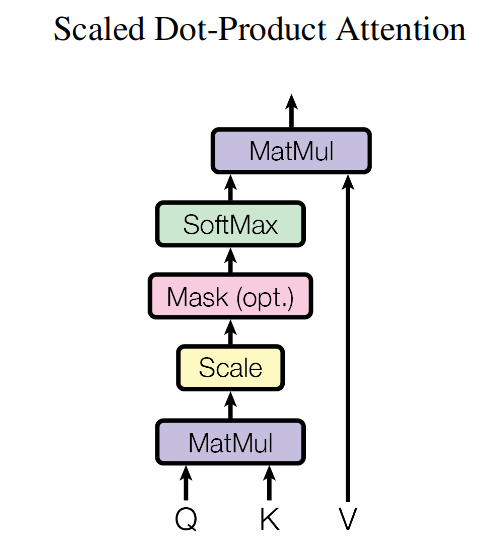
\includegraphics[width=0.25\textwidth]{dotproductAttn.png}
    \label{fig:dotproductAttn}
  }
  \subfloat[Multi-Head Attention]
  {
    \centering
    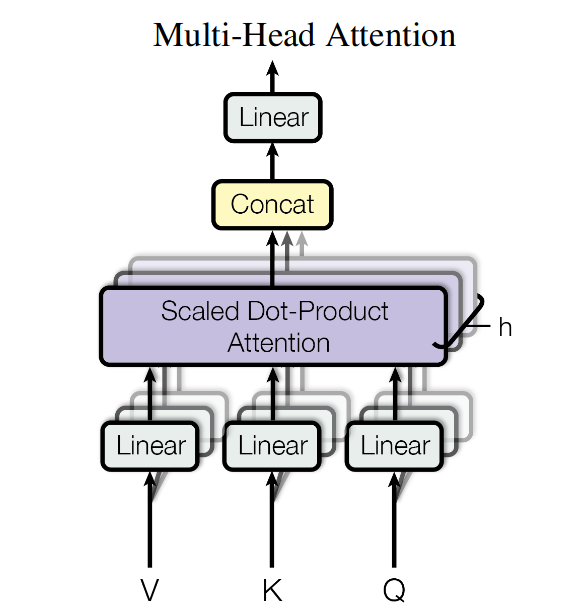
\includegraphics[width=0.25\textwidth]{mulheadAttn.png}
    \label{fig:mulheadAttn}
  }
  \subfloat[Transformerencoder]
  {
    \centering
    \includegraphics[width=0.25\textwidth]{Transformerencoder.png}
    \label{fig:Transformerencoder}
  }
  \subfloat[Atnal]
  {
    \centering
    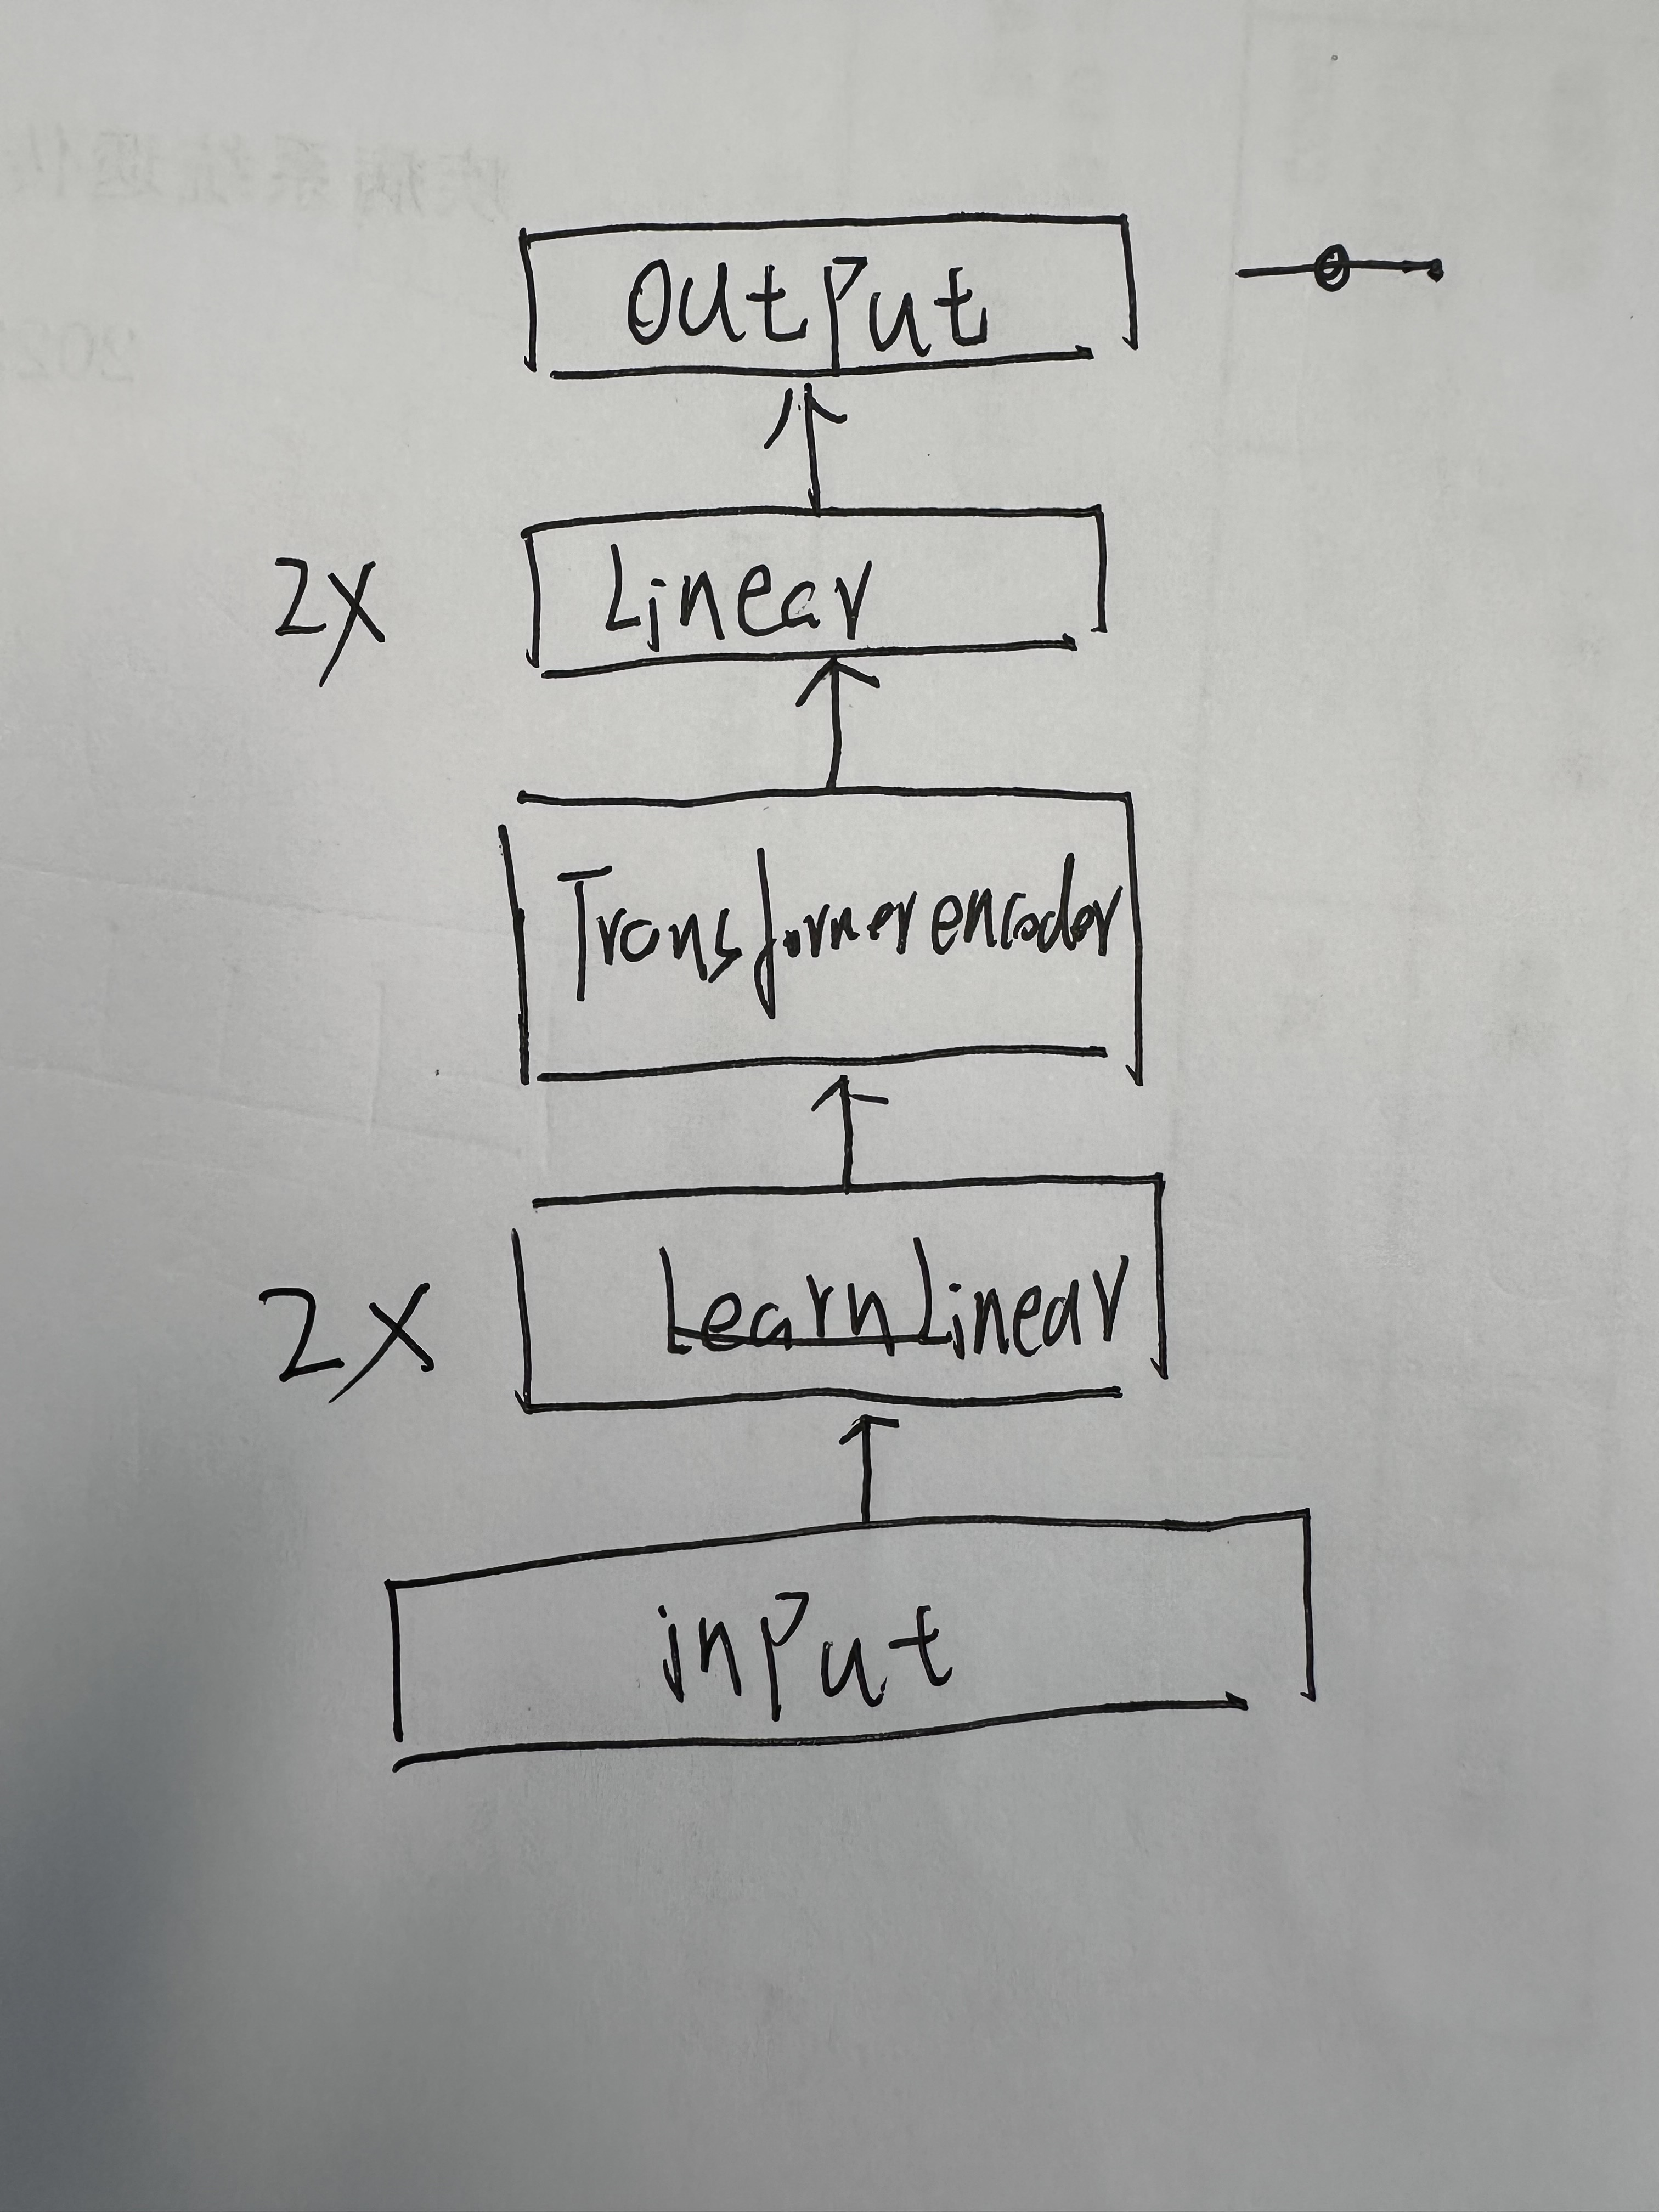
\includegraphics[width=0.25\textwidth]{model.png}
    \label{fig:model}
  }
\caption{Model}
\label{fig:Atnal}
\end{figure}

\textbf{Architecture of Atnal}: Atnal adopts an encoder-decoder architecture, 
to proceed efficient unsupervised learning and nonlinear 
dimensionality reduction using neural networks.  
The encoder, composing a Multilayer Perceptron (MLP) and a Transformerencoder \cite{vaswani2017attention}
(Figure \ref{fig:Transformerencoder}), 
maps an input sequence of symbol representations ( $x^{(1)}, ..., x^{(n)}$) 
to a sequence of continuous representations ( $z^{(1)}, ..., z^{(n)}$). 
It is used as a recognition model to 
infer an approximate estimate of the true but intractable distribution of the latent 
variable $z$ underlying the complex high-dimensional MSI data.
The decoder, a MLP, generates an output sequence ( $y^{(1)}, ..., y^{(n)}$) 
from ( $z^{(1)}, ..., z^{(n)}$). 
The decoder is used as a generative model to reconstruct the data by solely 
utilizing the encoded features ( $z^{(1)}, ..., z^{(n)}$). Both the parameters 
of the recognition model (encoder) and the generative model (decoder)
are jointly optimized and computed from the parameters of Atnal. As thus, the data flow of 
Atnal is as following:
\begin{equation}
  \begin{minipage}[c]{0.80\linewidth}
    \centering
    encoder($X$) = Transformerencoder($MLP_e$($X$)) \\
    Atnal($X$)=$MLP_d$(encoder($X$)) \\
  \end{minipage}
  \label{eqn:Atnal}
\end{equation}
where $X=( x^{(1)}, ..., x^{(n)})$. Transformerencoder will be introduced later. $MLP_e$ and $MLP_d$ are two different 
Multilayer Perceptrons mentioned in encoder and decoder, respectively.


\textbf{Transformerencoder}: Here we introduce the Transformerencoder in details, starting from the 
the fundamental module: Scaled Dot-Product Attention (Figure \ref{fig:dotproductAttn}) \cite{vaswani2017attention}.  
Its input consists of queries ($Q'$) and keys ($K'$) 
 of dimension $n \times d_k$, and values ($V'$) of  dimension $n \times d_{v}$. 
As introduced in [], we calculate the dot products of the
query with all keys, divide each by $\sqrt{d_{k}}$, and apply a softmax function to obtain the weights on the values. 
Consequently, the output of Scaled Dot-Product Attention can be given by
\begin{equation}
  \begin{minipage}[c]{0.80\linewidth}
    \centering
    Attention(Q',K',V')=Softmax($\frac{Q'K'^T}{\sqrt{d_{k}}}$)$V'$.
  \end{minipage}
  \label{eqn:Attention}
\end{equation}

The Scaled Dot-Product Attention is the kernel of Multi-Head Attention, as illustrated in Figure \ref{fig:mulheadAttn}. 
Using queries ($Q$), keys ($K$) and values ($V$) with dimension of $n \times d_{model}$ (different from $Q'$,$K'$,$V'$ mentioned earlier) as inputs,
the Multi-Head Attention allows Atnal to jointly attend to information from different representation subspaces 
at different positions. The queries, 
keys and values are projected  $h$ times by distinct, learned linear projections (in Figure \ref{fig:mulheadAttn})
to $d_k$, $d_k$ and $d_v$ dimensions, respectively. 
As a result, the data flow of Multi-Head Attention can be expressed as follows:
\begin{equation}
  \begin{minipage}[c]{0.80\linewidth}
    \centering
    MultiHead($Q$,$K$,$V$)= Concat($head_1$,$head_2$,...,$head_h$)$W^O $              \\
  \end{minipage}
  \label{eqn:MultiHeadAttn}
\end{equation}
where $W_i^O \in \mathbb{R}^{hd_v \times d_{model}}$ and 
\begin{equation}
  \begin{minipage}[c]{0.80\linewidth}
    \centering
    $head_i$ = Attention($QW_i^Q,KW_i^K,VW_i^V$) \,\,(Eq.~\ref{eqn:Attention})
  \end{minipage}
\end{equation}
Where the projections are parameter matrices 
$W_i^Q \in \mathbb{R}^{d_{model} \times d_k}$,
$W_i^K \in \mathbb{R}^{d_{model} \times d_k}$, and
$W_i^V \in \mathbb{R}^{d_{model} \times d_v}$. 
Throughout of this paper of this paper, we employ h = 8 parallel attention heads. Moreover, 
we select $d_k$ = $d_v$ = $d_{model}/h$ = 32 for each of these heads. 

Finally, the transformerencoder is structured by using two sub-layers. The first sub-layer 
consists of a multi-head self-attention mechanism, 
while the second sub-layer is a simple, fully connected feed-forward network (FFN). 
To ensure information flow smooth , 
We adopt a residual connection \cite{he2016deep} around each of the two sub-layers, 
followed by layer normalization \cite{hochreiter2001gradient}.
In general, the data flow from the input
of the Transformerencoder to its output is as fllows:
\begin{align}
  Q,K,V &= \text{input} \cdot \begin{bmatrix} W^1,W^2,W^3 \end{bmatrix} \\
  \text{output}_{\text{mul}} &= \text{LayerNorm}(\text{Residual}([Q,K,V],\text{MultiHead})) \\
  \text{output} &= \text{LayerNorm}(\text{Residual}(\text{output}_{\text{mul}},\text{FFN}))
\end{align}
where $input $ is calculated using the TIC-normalized spectra , and $W^1,W^2,W^3 \in \mathbb{R}^{d \times d_{model}}$  
are parameter matrices of three linear neural networks determined by 
backpropagation, and the function $\mathrm{Residual}(X,\text{sublayer})$ is:
\begin{align}
 \mathrm{Residual}(X,\text{sublayer}) = X + \text{sublayer}(X)
\end{align}

\textbf{Loss function}: In view of the fact that the reconstructed MSI data 
$Y = ( y^{(1)}, ..., y^{(n)})$ is a sparse matrix, 
the dissimilarity between Y and the input data $X=( x^{(1)}, ..., x^{(n)})$ 
can be computed as the error of a multi-classification problem. 
Here the dissimilarity is the loss function of Atnal, given by 
\begin{equation}
  \text{Loss} =\frac{1}{n} \sum_{i=1}^{n}H(X^{(i)}|Y^{(i)})
  \label{eqn:loss function}
\end{equation}
where $H$ (categorical cross-entropy loss 
 \cite{kingma2013auto}) is
\begin{equation}
  \begin{aligned}
    H(P^{*}|P) &= -\sum_{i}^{}P^{*}(i)\log P(i)      
  \end{aligned}
\end{equation}
where $P*$ and $P$ represent the true class distribution ($X^{(i)}$) and 
predicted class distribution ($Y^{(i)}$), respectively.

 
\subsection{Employ encoded features to identify biomarkers}
The encoded features represent the learned nonlinear manifold in 
lower-dimensional space, which can 
promote the visualization 
and extraction of molecular patterns from original high-dimensional data.
The inherent complexity of the 
original high-dimensional data is significantly reduced, which makes 
it possible to apply straightforward clustering algorithms such 
as the Gaussian-mixture 
model (GMM) \cite{reynolds2000speaker}. The GMM clustering result exhibits distinct 
clusters corresponding to specific regions on tissues. 
For better performance of clustering, the users have the flexibility to 
determine the number of clusters (k) for the GMM algorithm. 
Subsequently, a cluster of interest is selected for correlation 
analysis, which aims to determine a few colocalized m/z 
peaks associated with high Pearson correlation coefficients. 
This correlation analysis further enhances the interpretation of 
the relation between molecular patterns 
and the corresponding mass spectrometry imaging (MSI).

To identify biomarkers,  
initially, the determined m/z values are inputted into a 
comprehensive database of human metabolites, the Human 
Metabolome Database (HMDB). 
The compound, matched with an error of 5 ppm, is considered as a
potential metabolite for the corresponding m/z value. 
In case a m/z value does not match any human metabolite in the HMDB, 
then this particular m/z value will be further 
entered into the LIPID MAPS® Structure Database (LMSD) and 
MetaboAnalyst Database
for metabolite identification. Here, the tolerance window 
also remains at 5 ppm. 
If none of the three aforementioned databases 
can be used to find a match for a given m/z value, then this m/z 
value will be represented only by its m/z value, 
indicating that no known metabolite can be found for this specific value. 
\subsection{Code Availability}
The source code is available 
at GitHub (\href{https://github.com/AmFe-GH/Atnal}{https://github.com/AmFe-GH/Atnal}). 
As mentioned previously, the used datasets are assessible at 
\href{https://www.metabolomicsworkbench.org}{https://www.metabolomicsworkbench.org} and 
\href{https://doi.org/10.21228/M8BM4Q}{https://doi.org/10.21228/M8BM4Q}, respectively.

\section{RESULTS AND DISCUSSION}
\subsection*{Hyperparameters and implementation details}
The original MSI data is analyzed via Atnal, an encoder-decoder model 
based on attention mechanism and MLP 
(Multi-Layer Perceptron), as depicted in Figure ?. 
The proposed 
neural network architecture is comprised of six layers: an input 
layer ($L_1$), four hidden layers ($h_2$, $h_3$, $h_4$ and $h_5$), 
and an output layer ($L_6$). 
The number of artificial neurons of $L_1$ or $L_6$ 
is the same as that of the m/z  bins. The number of artificial neurons of 
hidden layers $h_2$, $h_3$, $h_4$ and $h_5$ 
is 512, 256, 256, and 512, respectively. 
The hidden layer $h_4$ captures the encoded features that represent 
the nonlinear dimensionality reduction 
of original MSI data compressed into
a 256-dimensional space. Layers $h_2$, $h_3$, and $h_5$
are performed by Batch normalization on their output. Further, 
the rectified linear unit \cite{nair2010rectified} (ReLU) function is used for neuron activation 
in the output of hidden layers $h_2$ and $h_5$. As for the output layer $L_6$, its neurons
are activated by the softmax function. 

Form a macro view in Atnal, the unsupervised learning process involves minimizing 
the reconstruction error between the original and predicted data. 
(The minimization is realized through  
optimizing the cost function modeled as the marginal likelihood and
calculated via categorical cross-entropy.); The Adam stochastic gradient optimizer 
is employed with a learning rate of 0.0002, in which the training is performed 
on minibatches consisting of 512 spectra for a total of 30 epochs. 
\subsection{Analysis of the 2D FT-ICR MSI data 
of prostate cancer tissue}

Aiming to validate the efficacy of Atnal in encoding features and reconstructing 
original data, we apply it in analyzing the entire dataset of prostate cancer tissue firstly. 
The results are presented in Figure \ref{fig:Training_pro},

The neural network employs unsupervised learning in an iterative fashion to 
minimize the reconstruction loss. As depicted in  Figure \ref{fig:loss_pro},
the optimizer achieves convergence in fewer than 
10 epochs, with a total running time of approximately 6 minutes. 
The encoded features, illustrated in  Figure \ref{fig:encoder_feature_2D_train_pro}, 
serve as a nonlinear embedding that facilitates visualization and reveals 
molecular patterns within a compressed  
representation of the original high-dimensional data.
The generative model reconstructs the originald data by only using 
these 256 dimensional encoded features.The overall loss 
of mean squared error (MSE) is $7  \times 10^{-9}$ between 
the normalized spectra of the 
original and predicted data. In order to visually 
demonstrate the quality of the reconstructed MSI data, we present the spatial
distributions of several selected spectra from both the original and 
predicted data in Figure \ref{fig:spesific_restruct_train_pro}, \ref{ori_pre}. 
The high similarity between these spectra is treated  as a 
reflection of the high quality of the estimation. 


The histopathological annotation of the prostate tumor regions reveals 
a Gleason score (GS) of (3 + 4) = 7 (Figure \ref*{fig:op_pro}) \cite{gleason1974prediction}. 
The understanding of molecular patterns underlying 
the annotated histopathological tumor region could contribute to the development 
of molecular diagnostics. The encoded features are clustered by the Gaussian-mixture 
model (GMM) with k-clusters (k = 17) (Figure \ref*{fig:clusters_pro}) .
Apparently, the light-blue cluster ? represents a molecular-based tumor 
pattern that matches with the histologically annotated tumor regions.

This molecular-based tumor cluster is selected (Figure \ref*{fig:selected_cluster_pro}) 
Then, we can find the ion 
feature m/z 739.4664 ± 0.001 with a Pearson correlation coefficient of 0.7 is 
tentatively assigned to ? C39H73O8P by searching the Human Metabolome Database (HMDB)40 
based on the accurate mass and with a tolerance window of 1.44 ppm, m/z 
985.5567 ± 0.001 with a correlation coefficient of 0.65 was tentatively identified 
as PIP(P-42:6) with an error of -0.14 ppm, and m/z 738.4548 ± 0.001 with a correlation 
coefficient of 0.64 was tentatively identified as PICer(t30:2) 
with an error of 0.53 ppm. A list of the top determinant m/z values for this tumor 
cluster with tentative molecular 
assignments are presented in Supplementary Table 1.

Among 15 m/z values with top-ranked correlation coefficients, 
7 of them are successfully identified within a tolerance window of 5 ppm. 
For example, the m/z value 774.5983 
indicates 16 potential phosphatidylcholine 
and phosphatidylethanolamine metabolites, including 
1-Pentadecanoyl-2-eicosenoyl-sn-glycero-3-phosphocholine, 
1-Eicosenoyl-2-pentadecanoyl-sn-glycero-3-phosphocholine, 
1-Myristoyl-2-nervonoyl-sn-glycero-3-phosphoethanolamine,  
% 1-Myristoleoyl-2-lignoceroyl-sn-glycero-3-phosphoethanolamine, 
% 1-Palmitoyl-2-erucoyl-sn-glycero-3-phosphoethanolamine, 
% 1-Palmitoleoyl-2-behenoyl-sn-glycero-3-phosphoethanolamine, 
% 1-Stearoyl-2-eicosenoyl-sn-glycero-3-phosphoethanolamine, 
% 1-Vaccenoyl-2-arachidonyl-sn-glycero-3-phosphoethanolamine, 
% 1-Oleoyl-2-arachidonyl-sn-glycero-3-phosphoethanolamine, 
% 1-Arachidonyl-2-vaccenoyl-sn-glycero-3-phosphoethanolamine, 
% 1-Arachidonyl-2-oleoyl-sn-glycero-3-phosphoethanolamine, 
% 1-Eicosenoyl-2-stearoyl-sn-glycero-3-phosphoethanolamine, 
% 1-Behenoyl-2-palmitoleoyl-sn-glycero-3-phosphoethanolamine, 
% 1-Erucoyl-2-palmitoyl-sn-glycero-3-phosphoethanolamine, 
% 1-lignoceroyl-2-myristoleoyl-sn-glycero-3-phosphoethanolamine, 
and 1-Nervonoyl-2-myristoyl-sn-glycero-3-phosphoethanolamine. 
Abnormal phospholipid metabolism is a key indicator of tumor. 
These phosphatidylcholine and 
phosphatidylethanolamine metabolites, as the products of phospholipid metabolism, 
play crucial roles in maintaining cellular 
membrane integrity and regulating lipid-dependent signaling pathways. 
The functions of phosphatidylcholines and phosphatidylethanolamines in the 
prostate cancer are also reported in several studies.




During the compound matching, a few signal molecules related to 
fatty acid metabolism are also discovered, such as m/z 762.5862 and m/z 804.6077. 
Among them, the m/z 804.6077 
is identified as 12 potential compounds which belong to the class 
of glycerophospholipids. They include 
1-hexadecyl-2-(11Z-docosenoyl)-glycero-3-phosphoserine, 
1-octadecyl-2-(11Z-eicosenoyl)-glycero-3-phosphoserine,
1-eicosyl-2-(9Z-octadecenoyl)-glycero-3-phosphoserine,
1-eicosyl-2-(6Z,9Z,12Z-octadecatrienoyl)-glycero-3-phospho-(1'-sn-glycerol) and so on. 
All these compounds are 
previously identified in prostate cancer samples in the human metabolomics database, 
Metabolomics Workbench (https://www.metabolomicsworkbench.org/), 
with study IDs ST000784 and ST001133. 
As for the m/z 762.5862, it is identified as a neutral glycosphingolipids compound, and the 
best match is found with N-(docosanoyl)-1-beta-glucosyl-4E,6E-pentadecasphingadienine in human 
metabolites, with an error of 1.00 ppm. 
For more information on compound identification, please refer to Supplementary Table 1.
 \begin{figure}[htbp]
  \centering
    \subfloat[Traing loss]
    {
      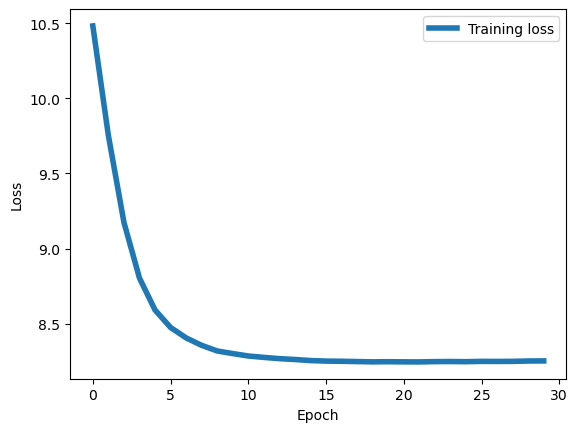
\includegraphics[width=0.5\textwidth]{loss_pro.png}
      \label{fig:loss_pro}
    }
    \subfloat[Ecoder features]
    {
      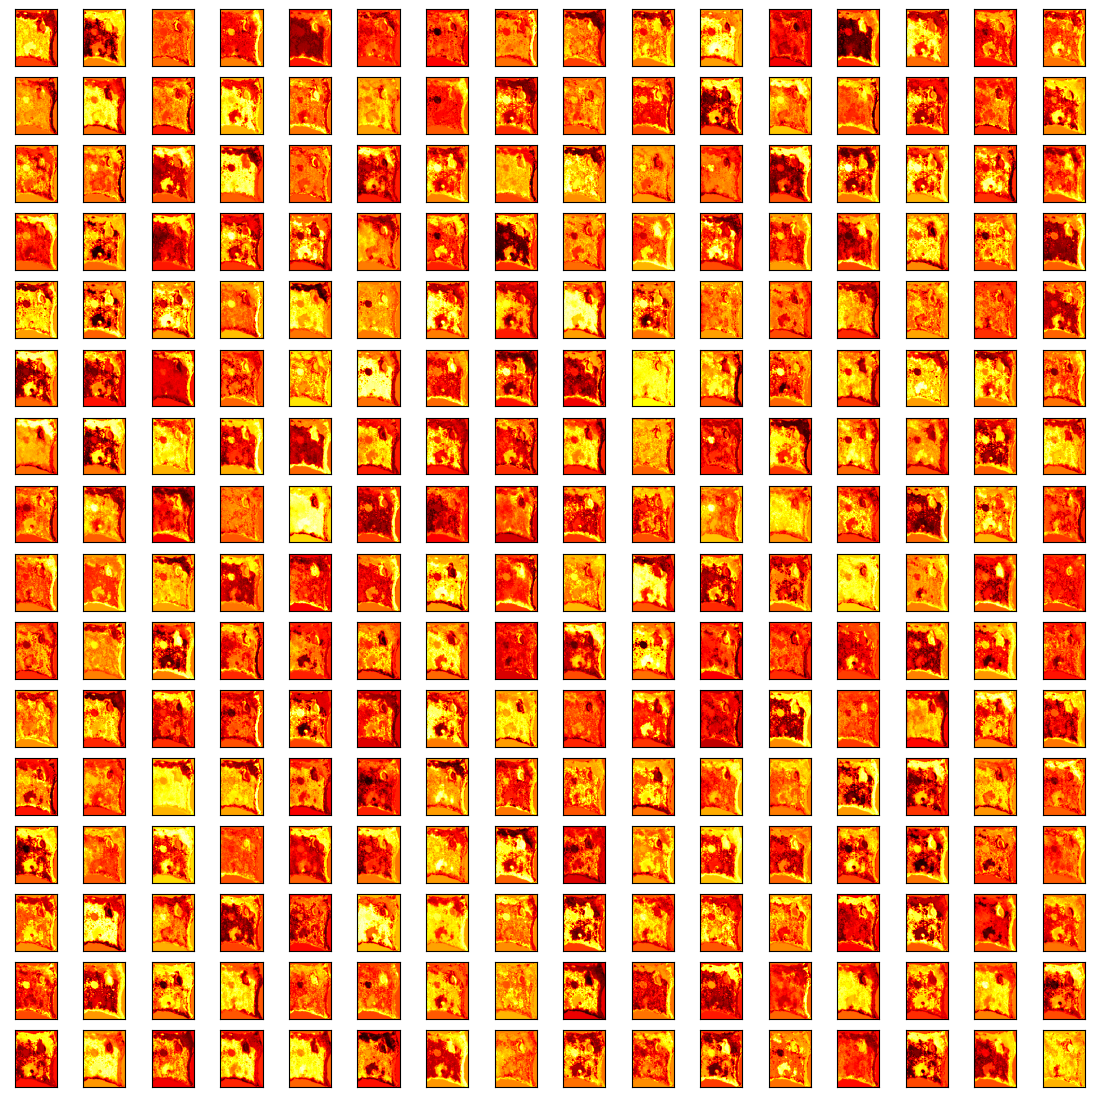
\includegraphics[width=0.38\textwidth]{pic/encoder_feature_2D_train_pro.png}
      \label{fig:encoder_feature_2D_train_pro}
    }
  
  \subfloat[Restruct specific spectra]
  {
    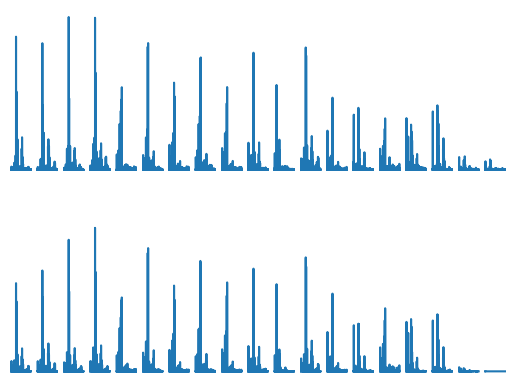
\includegraphics[width=\textwidth,height=0.2\textheight]{spesific_restruct_train_pro.png}
    \label{fig:spesific_restruct_train_pro}
  }

  \subfloat[clustering result]
  {
    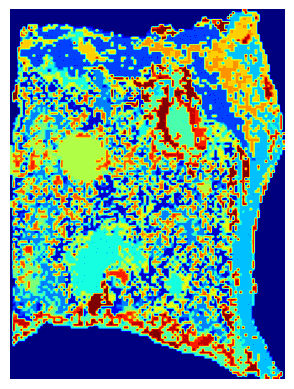
\includegraphics[width=0.2\textwidth]{./pic/prostate/clusters.png}
    \label{fig:clusters_pro}
  }
  \subfloat[selected cluster]
  {
    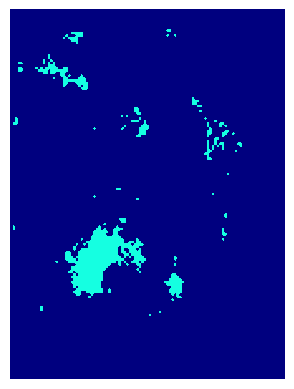
\includegraphics[width=0.2\textwidth]{./pic/prostate/selected.png}
    \label{fig:selected_cluster_pro}
  }  
  \subfloat[selected m/z pattern]
  {
    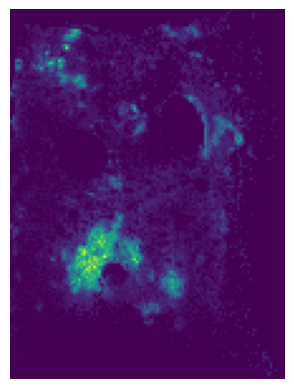
\includegraphics[width=0.2\textwidth]{./pic/prostate/selected_mz.png}
    \label{fig:selected_mz_pro}
  }  
  \subfloat[histopathological annotation]
  {
    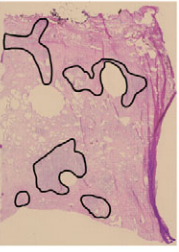
\includegraphics[width=0.185\textwidth]{./pic/prostate/op.png}
    \label{fig:op_pro}
  }
\caption{Training phase}
\label{fig:Training_pro}
\end{figure}
\subsection{Analysis of the 3D DESI MSI data of colorectal adenocarcinoma dataset}
Here, we apply Atnal to reconstruct a 3D MSI volume from a human colorectal 
adenocarcinoma specimen: 26 consecutive 
(acquired at every 100 $\mu$m) 10 $\mu$m 
thickness tissue sections. 
To reduce the impact of imbalanced data splitting on model loss, 
we implemente K-fold cross-validation during the process of the model 
training (Figure \ref{fig:Training}), in which 26 tissue sections 
from the colorectal 
carcinoma specimen are divided into K groups (Figure \ref{fig:k_fold}). 
Each time one group is designated as the testing set, while the other 
groups are regarded as the training set. This is repeated K times, 
ensuring that each group can serves as the testing set at least once, and providing a 
comprehensive evaluation of model performance.

In the MSI data of colorectal adenocarcinoma
dataset, K is selected as 5 for the cross-validation. During 
each iteration of the 5-fold cross-validation, the data from 4 randomly selected groups, 
comprised of 20 tissue sections with a total of 93,482 spectra, 
are used to train Atnal. 
The training process of Atnal becomes convergent after approximately 10 epochs, 
as depicted in Figure (Figure \ref{fig:loss}). The total running time costed for this 
convergence is approximately 1.5 minutes. Based on the encoded features derived by 
the encoder of Atnal, the original spectral are 
reconstructed with an overall mean squared training error of $1.3 \times 10^{-7}$. 

Once the model training is completed, its performance is further evaluated by 
using the remaining 6 tissue sections with 29,006 spectra (testing set).
The spectra in the same batch 
are loaded into the memory and analyzed by Atnal. 
It takes approximately 4 s for the encoder of Atnal
to predict the encoded features and another 3 s for the decoder 
to reconstruct the data. 
The strong resemblance observed between the original and reconstructed spectra, 
as shown in \ref{fig:spesific_restruct_train}, indicates that the encoder 
successfully captures the intricate features present in the nonlinear 
manifold of the original high-dimensional data.

The encoded features as Figure \ref{fig:encoder_feature_3D_test}, represents a 
256-dimensional nonlinear embedding of the original high-dimensional testing data. 
The overall mean square testing error between the reconstructed and original data
is  $2.1 \times 10^{-7}$. 
The testing results, 5 GMM clusters, of the encoded features, carries significant 
implication. 2 of 5 GMM clusters associate with tumor and connective tissues. 
This implication is consistent with the results in previous studies 
\cite{abdelmoula2018interactive} \cite{oetjen2015benchmark} 
and images of the H\&E stained tissue sections,  see 
Figure \ref{fig:clustering_1} \ref{fig:clustering_11} \ref{fig:clustering_13}. 

The encoded features are then clustered by GMM (K = 5), forming five clusters, 
and two of them (cluster 3 and cluster 5) show
a high degree of consistency with 
histological evaluation (H\&E) as illistrated in Figure \ref{fig:clustering_4}. 
These two clusters correlate with 
the ions at m/z 720.49 ± 0.1 and m/z 766.53 ± 0.1, of which the  pearson correlation 
values are 0.7761 and 0.746, respectively.
Moreover, this result is consistent with the observation that 
the intensities of the ions at m/z 720.49 ± 0.1 and m/z 766.53 ± 0.1 are 
particularly high in the tumor and connective tissue, respectively. 

\begin{figure}[htbp]
  \centering
  \begin{minipage}[c]{0.44\textwidth}
    % \flushleft 
    \subfloat[Training/Testing set split]
    {
      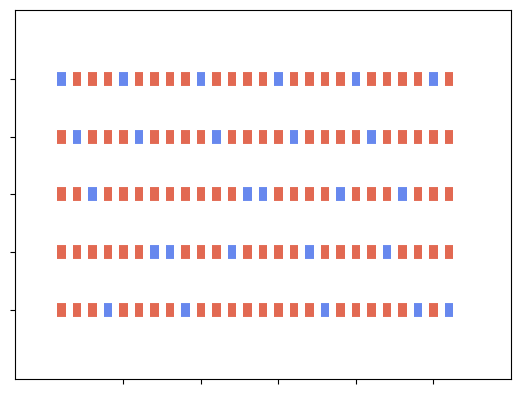
\includegraphics[width=0.94\textwidth]{k_fold.png}
      \label{fig:k_fold}
    }\\
    \vspace{-5pt}
    \subfloat[Traing loss]
    {
      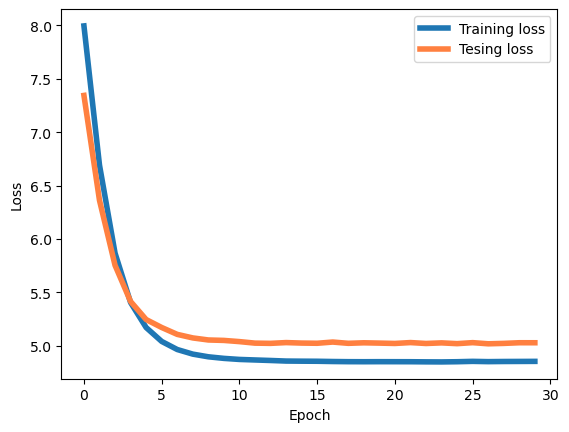
\includegraphics[width=0.77\textwidth]{loss.png}
      \label{fig:loss}
    }
  \end{minipage}
  \hfill
  \begin{minipage}{0.55\textwidth}
    \subfloat[Ecoder features]
    {
      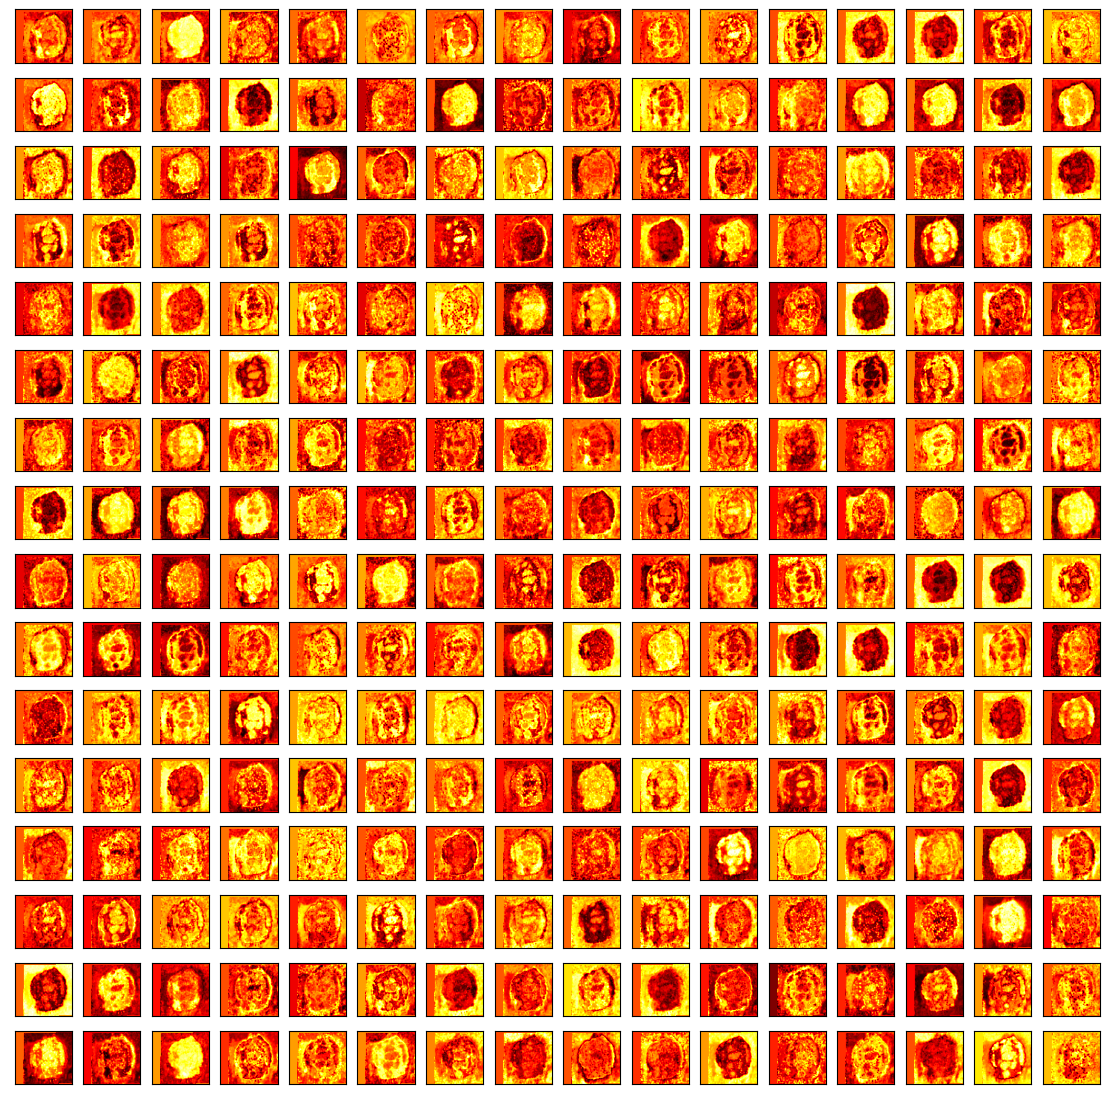
\includegraphics[width=\textwidth]{pic/encoder_feature_3D_train.png}
      \label{fig:encoder_feature_3D_train}
    }
  \end{minipage}
\vspace{-10pt}
  
  \subfloat[Restruct specific spectra]
  {
    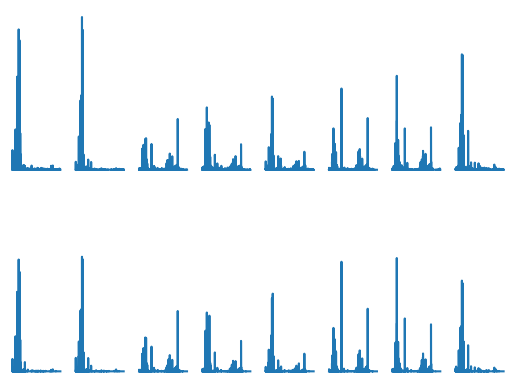
\includegraphics[width=0.5\textwidth,height=0.2\textheight]{spesific_restruct_train.png}
    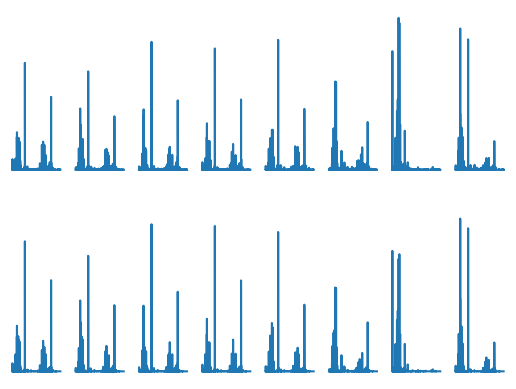
\includegraphics[width=0.5\textwidth,height=0.2\textheight]{spesific_restruct_test.png}
    \label{fig:spesific_restruct_train}
  }

  \subfloat[Section4]
  {
    
\includegraphics[width=0.2\textwidth,height=0.137\textheight]{../Results_CV/Section3/clusters .png}
    
\includegraphics[width=0.2\textwidth,height=0.137\textheight]{../Results_CV/Section3/cluster35.png}
    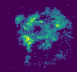
\includegraphics[width=0.2\textwidth,height=0.137\textheight]{../Results_CV/Section3/cluster3.png}
    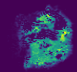
\includegraphics[width=0.2\textwidth,height=0.137\textheight]{../Results_CV/Section3/cluster5.png}
    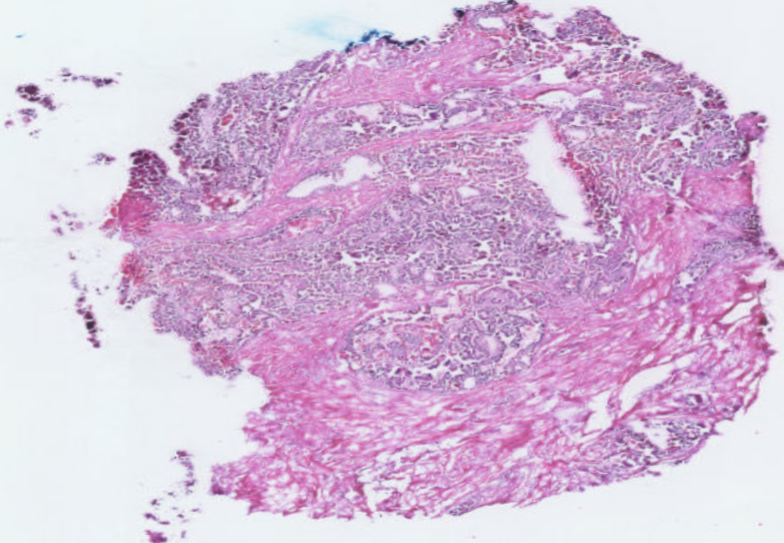
\includegraphics[width=0.2\textwidth,height=0.137\textheight]{../Results_CV/Section3/op.png}
    \label{fig:clustering_4}
  }
  % \subfloat[Section9]
  % {
  %   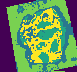
\includegraphics[width=0.2\textwidth,height=0.137\textheight]{../Results_CV/Section8/clusters .png}
  %   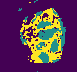
\includegraphics[width=0.2\textwidth,height=0.137\textheight]{../Results_CV/Section8/cluster35.png}
  %   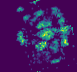
\includegraphics[width=0.2\textwidth,height=0.137\textheight]{../Results_CV/Section8/cluster3.png}
  %   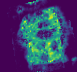
\includegraphics[width=0.2\textwidth,height=0.137\textheight]{../Results_CV/Section8/cluster5.png}
  %   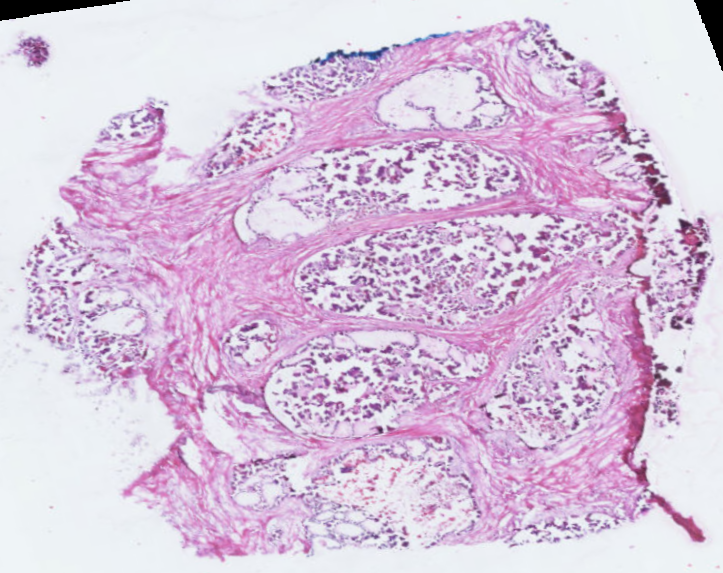
\includegraphics[width=0.2\textwidth,height=0.137\textheight]{../Results_CV/Section8/op.png}
  %   \label{fig:clustering_9} 
  % }

  % \subfloat[Section26]
  % {
  %   
\includegraphics[width=0.2\textwidth,height=0.137\textheight]{../Results_CV/Section25/clusters .png}
  %   
\includegraphics[width=0.2\textwidth,height=0.137\textheight]{../Results_CV/Section25/cluster35.png}
  %   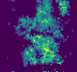
\includegraphics[width=0.2\textwidth,height=0.137\textheight]{../Results_CV/Section25/cluster3.png}
  %   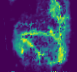
\includegraphics[width=0.2\textwidth,height=0.137\textheight]{../Results_CV/Section25/cluster5.png}
  %   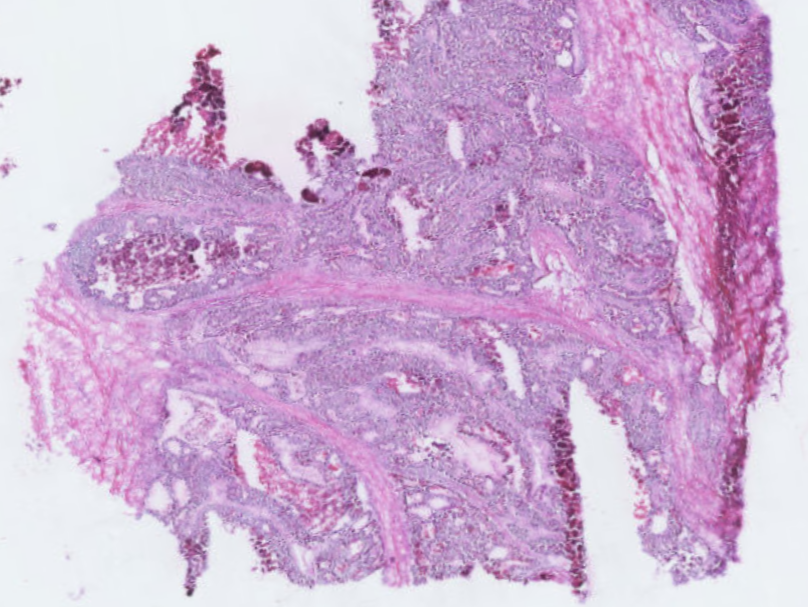
\includegraphics[width=0.2\textwidth,height=0.137\textheight]{../Results_CV/Section25/op.png}
  %   \label{fig:clustering_26} 
  % }
\caption{Training phase}
\label{fig:Training}
\end{figure}


14 m/z values are discovered 
strongly correlated with colorectal cancer. As checked with HMDB, LMSD, 
and MetaboAnalyst database, 
9 of 14 are successfully identified. For instance, m/z 858.5260627 
is identified as compounds belonging to the class of phosphatidylserines 
with an  tolerance window of 5 ppm, including 
1-(11Z,14Z-eicosadienoyl)-2-(4Z,7Z,10Z,13Z,16Z,19Z-docosahexaenoyl)-glycero-3-phosphoserine, 
1-(5Z,8Z,11Z,14Z-eicosatetraenoyl)-2-(7Z,10Z,13Z,16Z-docosatetraenoyl)-glycero-3-phosphoserine, 
1-(7Z,10Z,13Z,16Z-docosatetraenoyl)-2-(5Z,8Z,11Z,14Z-eicosatetraenoyl)-glycero-3-phosphoserine, 
and 1-(4Z,7Z,10Z,13Z,16Z,19Z-docosahexaenoyl)-2-(11Z,14Z-eicosadienoyl)-glycero-3-phosphoserine. 
It is speculated that they are related 
to the vigorous phospholipid metabolism of colorectal cancer cells. Nevertheless, 
there is no relevant report on phosphatidylserines compounds as colorectal cancer markers. 
For more details on the identification of these compounds, see Supplementary Table 2.
\begin{figure}[htbp]
  \centering
  \subfloat[Encoded features in testing set]
    {
      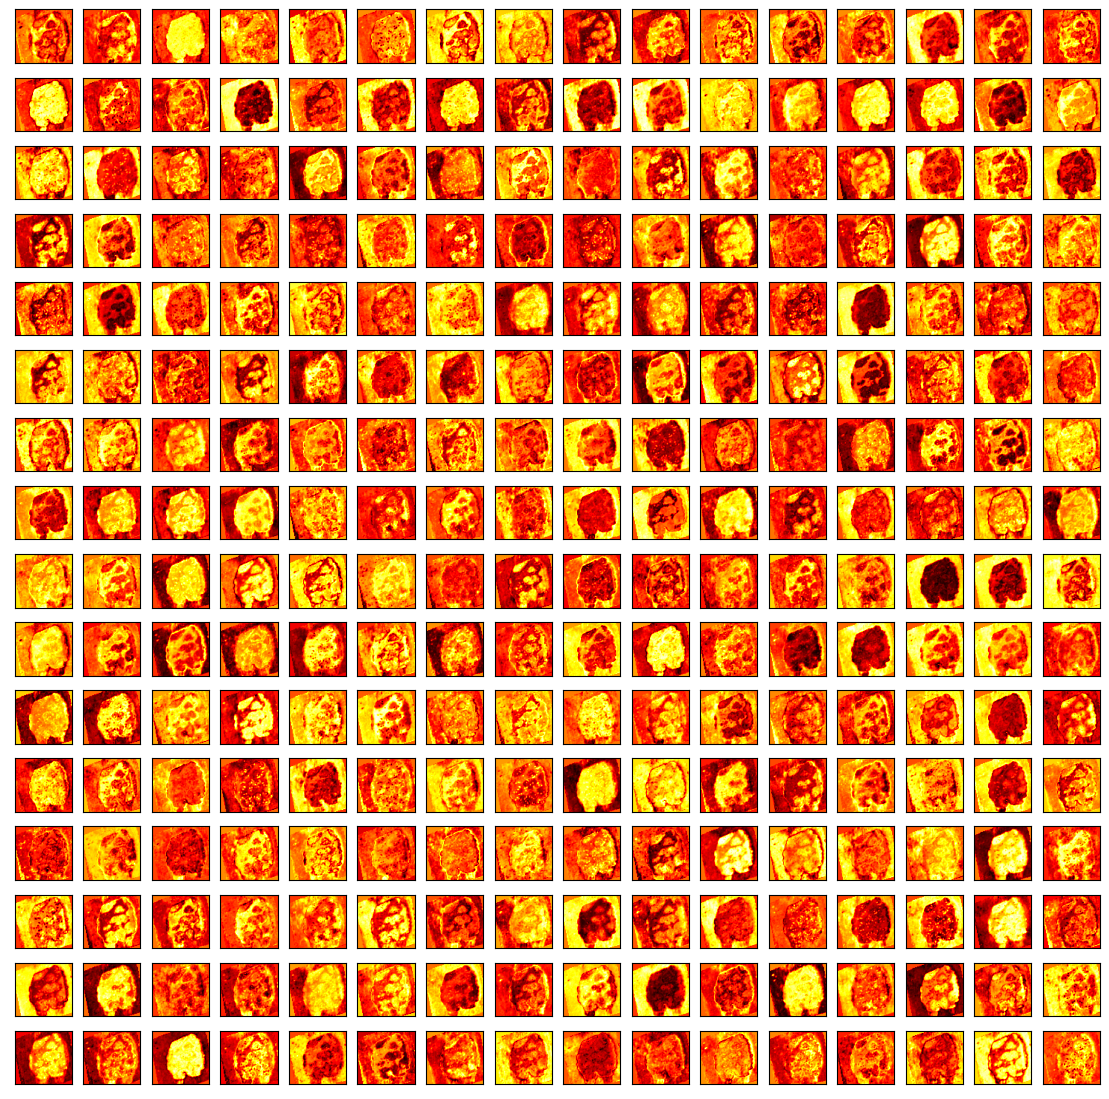
\includegraphics[width=0.6\textwidth]{pic/encoder_feature_3D_test.png}
      \label{fig:encoder_feature_3D_test}
    }
    \\
  \subfloat[Section 1]
  {
    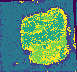
\includegraphics[width=0.2\textwidth,height=0.137\textheight]{../Results_CV/Section0/clusters .png}
    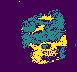
\includegraphics[width=0.2\textwidth,height=0.137\textheight]{../Results_CV/Section0/cluster34.png}
    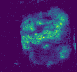
\includegraphics[width=0.2\textwidth,height=0.137\textheight]{../Results_CV/Section0/cluster3.png}
    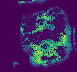
\includegraphics[width=0.2\textwidth,height=0.137\textheight]{../Results_CV/Section0/cluster4.png}
    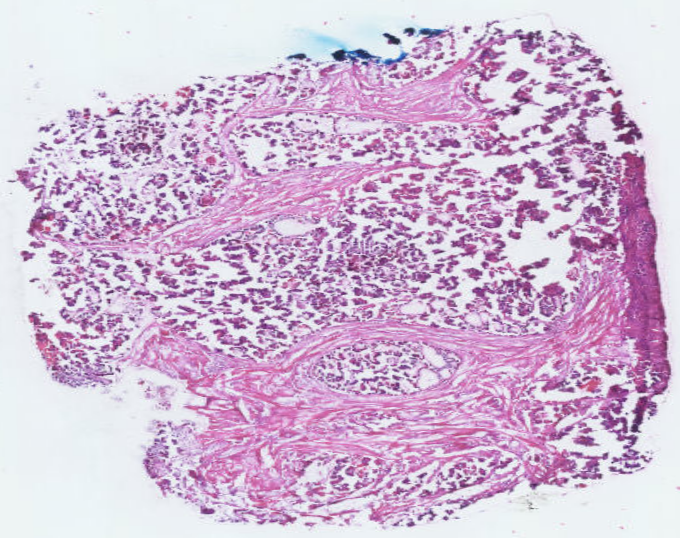
\includegraphics[width=0.2\textwidth,height=0.137\textheight]{../Results_CV/Section0/op.png}
    \label{fig:clustering_1}
  }

  \subfloat[Section 11]
  {
    
\includegraphics[width=0.2\textwidth,height=0.137\textheight]{../Results_CV/Section10/clusters .png}
    
\includegraphics[width=0.2\textwidth,height=0.137\textheight]{../Results_CV/Section10/cluster34.png}
    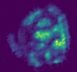
\includegraphics[width=0.2\textwidth,height=0.137\textheight]{../Results_CV/Section10/cluster3.png}
    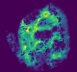
\includegraphics[width=0.2\textwidth,height=0.137\textheight]{../Results_CV/Section10/cluster4.png}
    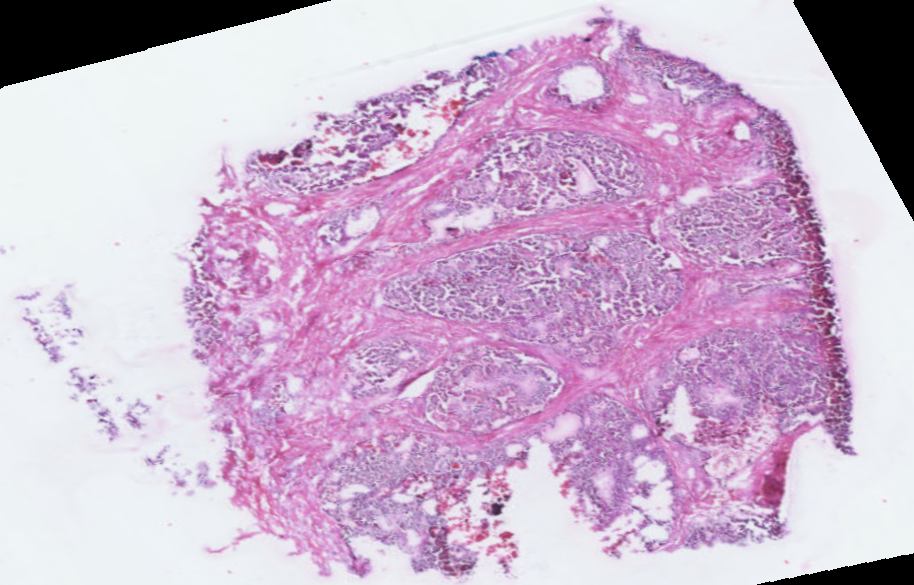
\includegraphics[width=0.2\textwidth,height=0.137\textheight]{../Results_CV/Section10/op.png}
    \label{fig:clustering_11}
  }

  \subfloat[Section 13]
  {
    
\includegraphics[width=0.2\textwidth,height=0.137\textheight]{../Results_CV/Section12/clusters .png}
    
\includegraphics[width=0.2\textwidth,height=0.137\textheight]{../Results_CV/Section12/cluster34.png}
    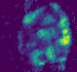
\includegraphics[width=0.2\textwidth,height=0.137\textheight]{../Results_CV/Section12/cluster3.png}
    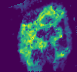
\includegraphics[width=0.2\textwidth,height=0.137\textheight]{../Results_CV/Section12/cluster4.png}
    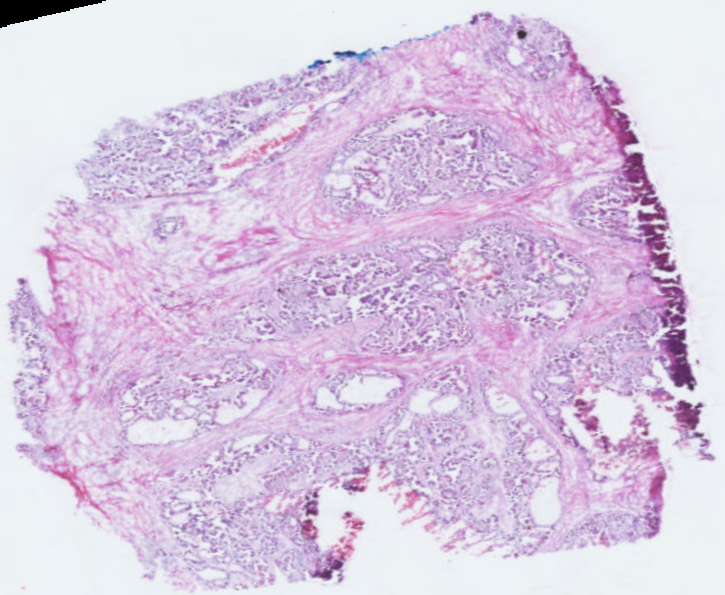
\includegraphics[width=0.2\textwidth,height=0.137\textheight]{../Results_CV/Section12/op.png}
    \label{fig:clustering_13}
  }
\caption{Testing phase}
\label{fig:Testing}
\end{figure}




\subsubsection{Discussion}
In this study, a novel method called Atnal is developed 
for analyzing MSI data collected from different types of 
human tissues. It can be used to reveal heterogeneity in cancer 
tissues, discovering of 
cancer biomarkers, and assist in cancer clinical diagnosis.
In the following, we discuss the details of the training and application 
(dimension reduction and clustering) of Atnal.
\begin{figure}[htbp]
  \centering
  \begin{minipage}{0.46\textwidth}
    \subfloat[Pearson in msiPL and Atnal]{
      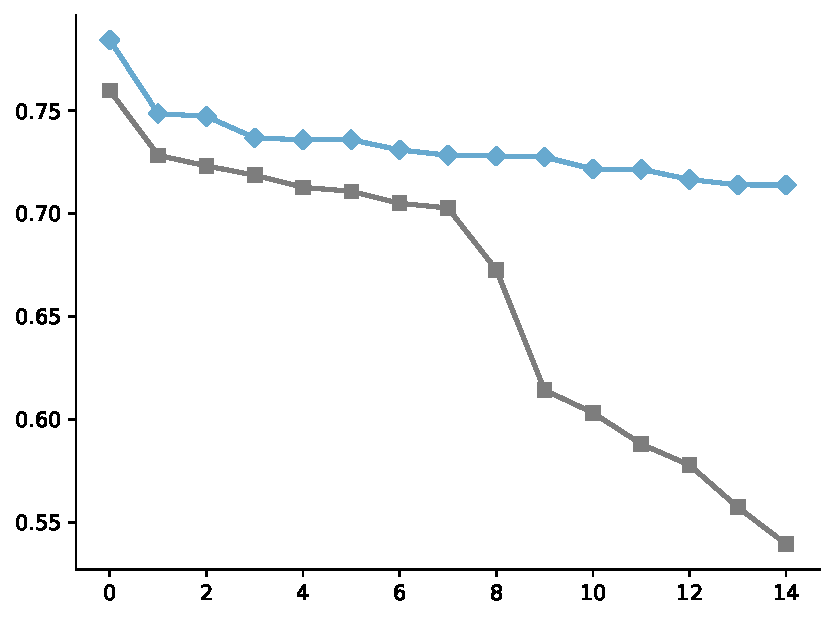
\includegraphics[width=\textwidth]{pic/pearson.pdf}
      \label{fig:Pearson_msiPL_Atnal}
    }
  \end{minipage}
  \begin{minipage}{0.51\textwidth}
    \subfloat[Loss of different models]
    {
    \includegraphics[width=\textwidth]{pic/loss.pdf}
    \label{fig:Loss in models}
    }
  \end{minipage}
  \subfloat
  {
    \includegraphics[width=0.3\textwidth]{./pic/coloractal/hist.pdf}
    \label{fig:hist}
  }
\caption{Quantitative comparative analysis of model performance}
\label{fig:model performance}
\end{figure}
\vspace{-10pt}

\textbf{Training}: During the training, self-supervised learning is employed to extract prior 
information from the raw data; 
ReLU activation functions are extensively 
adopted to introduce non-linearity; and Softmax 
activation functions are used  in the final output layer to 
ensure the reconstructed data values have the same range as 
normalized input, that is, from 0 to 1. 
The consistency of the value range between the input and output layers is 
crucial for minimizing the loss function expressed 
by Equation \ref{eqn:loss function}. 
Adopting the learning rate decay in self-supervised learning,
Atnal shows strong generalization and excellent performance on 
reconstructing original data, and avoid overfitting
the training data , as shown in Figure \ref{fig:loss}. 
Without manual feature 
engineering during mass spectrometry 
imaging data analysis , Atnal can accelerate the identification of 
biologically relevant ions and reduce the biases introduced 
by subjective factors, thereby promoting the process of 
biomarker discovery. 
The loss function is given by 
the categorical cross-entropy that assigns higher weights 
to non-zero data in the spectral data 
and makes Atnal more sensitive to the reconstruction of the original data. 
Atnal uses mini-batch training, which allows 
loading only a small portion of the spectral 
data into the graphics memory. This enables the Graphics Processing Units (GPUs) to process
large and complex datasets, and empowers Atnal to 
conduct single-precision floating-point training on a workstation 
with 64 GB of memory and 8 GB of graphics memory. 


As the kernel of Atnal, the attention mechanism simulates the human 
attention mechanism, and assist Atnal in focusing on 
relevant parts of the input sequence 
in the spectra by treating 
the intensity  
at different m/z values as the features of these spectra. Without any
positional information, the attention 
matrices between different spectra are  constructed  to discover the 
intrinsic correlations among these spectra. 
In a self-attention layer ($h_4$), the keys, values, and queries (mentioned 
in Equation \ref{eqn:MultiHeadAttn}) are all derived 
from the output of the previous layer ($h_3$) in the encoder. 
As a normal module used in deep neural networks, the residual connection module 
provides a direct flow of information from  layer $h_3$ to  $h_4$. 
To test the functions of the 
attention module and the residual connection module, we conduct an ablation experiment. 
As shown in Table \ref{tab:ablation_experiment}, 
using only one of the two modules results in a varying degree of 
decrease in model performance. 
Moreover, as a comparism, when we incorporate both the attention module and the 
residual connection module as sub-modules in Atnal, we can 
achieve the optimal results.

Now we analyze the reasons for the experiment result above. 
The attention module enables the model to learn the 
weights of different positions in the input, and allows for 
focusing on the spectra which located in the positions with high weights 
and  reducing the interference from the information with low weights. 
But, relying only 
on the attention module (without residual module) may lead 
to an excessive attention on some certain 
positions or features.
Similarly, the residual connection module may facilitate direct information 
propagation within networks and ?respond? to challenges from gradient 
vanishing and exploding, so as to reduce information loss in deep 
networks on one hand. On the other hand, only using the residual 
connection module may introduce 
too much information flow, which results in overreliance on previous 
layers and limits model stability and expressive capacity. 
As seen, integrating the residual connection module and the attention module 
contribute to a balance between these advantages and disadvantages, which benifits 
both the information transmission and selection, 
thus enhancing the overall performance.

% As for the learnable parameters of Atnal, their scale is huge: 
% 11.17 million, which makes Atnal a large model. Nonetheless, Atnal can be easily 
% trained. Specificly, Atnal converges in only 10 epochs, and it only take 
% less than 10 minutes for training.
% In comparism, the up-to-date neural-network-based method "msiPL" \cite{abdelmoula2021peak} 
% requires approximately 100 epochs. Note that
% the rapid convergence of Atnal is not acquired through a high learning 
% rate that may  lead to instability (oscillations of loss) in the later stages of training. 
% This is crucial for a reproducible and interpretable model.

When it comes to the performance of Atnal, comparing with that of other
methods (such as PCA, memory-efficient 
PCA, and Discrete Wavelet Transform (DWT) and PCA), 
as shown in Figure \ref{fig:Loss in models}, Atnal has smaller MSE than traditional 
PCA-based methods, and significantly lower MSE than other 
encoder-decoder-based methods (msiPL) by two orders of magnitude.
\begin{table}[htbp]
  \centering
  \caption{Comparison MSE of MSI data reconstruction using different methods}
  \label{tab:ablation_experiment}
  \begin{tabular}{cccc}
    \toprule
    & \textbf{PCA} & \textbf{msiPL} & \textbf{Atnal} \\
    \midrule
    \textbf{MSI Prostate Dataset} & $1.8 \times 10^{-2}$ & $6.9 \times 10^{-5}$ & $7.0 \times 10^{-9}$ \\
    \textbf{MSI Colorectal carcinoma Dataset} & $1.4 \times 10^{-1}$ & $1.6 \times 10^{-4}$ & $2.1 \times 10^{-7}$ \\
    \bottomrule
  \end{tabular}
\end{table}
\vspace{-10pt}
\begin{table}[htbp]
  \centering
  \caption{Ablation of Atnal with colorectal carcinoma dataset}
  \label{tab:ablation_experiment}
  \begin{tabular}{ccc}
    \toprule
    & \multicolumn{2}{c}{\textbf{Loss}} \\
    \cmidrule{2-3}
    \textbf{Experimental Condition} & \textbf{Training} & \textbf{Testing} \\
    \midrule
    \textbf{Base} & $1.567 \times 10^{-7}$ & $2.262 \times 10^{-7}$ \\
    \textbf{Base + Residual} & $2.02 \times 10^{-7}$ & $2.86 \times 10^{-7}$ \\
    \textbf{Base + Attention} & $4.2 \times 10^{-7}$ & $8.1 \times 10^{-7}$ \\
    \textbf{Base + Attention + Residual} & $\mathbf{1.41 \times 10^{-7}}$ & $\mathbf{2.119 \times 10^{-7}}$ \\
    \bottomrule
  \end{tabular}
\end{table}
\vspace{-10pt}
\begin{table}[htbp]
  \centering
  \caption{Dimensions of Each Layer}
  \begin{tabular}{cccccc}
    \toprule
    \textbf{$h_1$} & \textbf{$h_2$} & \textbf{$h_3$} & \textbf{$h_4$} & \textbf{$h_5$} & \textbf{$h_6$} \\
    \midrule
    m/z dimensions & 512 & 256 & 256 & 512 & m/z dimensions \\
    \bottomrule
  \end{tabular}
  \label{tbl:Dimensions of Each Layer}
\end{table}


\textbf{Application}: After the training, the original high-dimensional 
spectral data is encoded into 
low-dimensional features by the encoder of Atnal. 
The data complexity (for subsequent 
analysis) is reduced from tens of thousands dimensions 
to a 256 dimensions (Table \ref{tbl:Dimensions of Each Layer}). This avoids 
the curse of dimensionality problem commonly encountered in traditional machine 
learning methods.

The obtained encoded features are then fed into the 
GMM clustering algorithm.  
From the results shown in Figure \ref{fig:clusters_pro} 
\ref{fig:clustering_1} \ref{fig:clustering_11} \ref{fig:clustering_13}, 
it can be observed that the spectra  
corresponding to these cancer regions (annotated by pathologists) are 
easily clusted into the same group, and exhibit 
significant distinctions from other spectra (the spectra associated with non-cancer regions). 
Based on the observation, 
we further compute the correlation between each m/z dimension in the 
spectral data and the spectra in the cancer cluster, and identify a few number of m/z 
values that show high correlations with the cancer regions
(Figure \ref{fig:Pearson_msiPL_Atnal}).  

These identified m/z values can 
indicate potential biomarkers and be further used to search
corresponding substances in databases. In Figure \ref{fig:hist}, 
we conduct cross-validation analyses and obtain a list of the top 
100 m/z values based on their correlations. Among these values, there are 121 unique 
m/z peaks. Remarkably, 
80 (66\% of 121) are identified as stable, consistently 
detected across all cross-validation analyses. 

\section{Conclusion}
In this work, we develop a new approach, namely, 
Atnal, a generic neural-network-based method for the 
analysis of MSI data from different types of mass spectrometer and tissue type. 
And this method exhibits outstanding performance, showcasing its ability 
to capture the complex nonlinear manifold of spectral structures and 
its remarkable sensitivity to potential biomarkers. 

In this study, a novel method called Atnal is developed for analyzing MSI data collected from 
different types of human tissues. It can be used to reveal heterogeneity in cancer tissues, 
discovering of cancer biomarkers, and assist in cancer clinical diagnosis. In the following, we 
discuss the details of the training and application (dimension reduction and clustering) of 
Atnal. 

In conclusion, we have developed a novel method called Atnal, which effectively maps 
high-dimensional metabolomics data to a low-dimensional space with minimal 
loss ($2 \times 10^{-7} \sim 7 \times 10^{-9}$). The resulting encoded information represents the primary mass 
spectral features of the original MSI data, pointing to specific cancer biomarkers 
and aiding in clinical cancer detection and diagnosis. We trained the attention-based 
model Atnal and demonstrated its application in biomarker identification and cancer 
region recognition using metabolomics data from patients with prostate cancer and 
colorectal adenocarcinoma. We identified highly correlated biomarkers with cancer 
(highest Pearson correlation coefficient of 0.79) and accurately differentiated 
cancerous tissue from connective tissue (colorectal adenocarcinoma MSI dataset). 
n conclusion, Atnal is a novel approach that efficiently extracts key information 
from MSI mass spectral data and facilitates the utilization of the entire metabolome 
spectrum in AI-based clinical applications. However, this study has some limitations. 
The model training and validation were based on different parts of the same individual. 
To truly apply it in clinical settings, it is necessary to validate the model using 
multiple datasets collected from different individuals. Additionally, the workflow of 
Atnal is solely based on MSI intensity data, and incorporating spatial information may 
enhance the model. While Atnal was not specifically developed for a particular 
application, we believe this method opens new avenues for metabolomics-based clinical 
applications in various scenarios, including 
other biofluid types (e.g., urine) and clinical proteomics-based approaches.

\newpage
\begin{figure}[htbp]
  \centering
  \begin{minipage}[c]{0.9\textwidth}
  {
    % \includegraphics[width=0.19\textwidth]{pic/prostate/mz250.00154.png}
    % \includegraphics[width=0.19\textwidth]{pic/prostate/mz300.00015.png}
    % \includegraphics[width=0.19\textwidth]{pic/prostate/mz350.00183.png}
    % \includegraphics[width=0.19\textwidth]{pic/prostate/mz400.00262.png}
    % \includegraphics[width=0.19\textwidth]{pic/prostate/mz449.99185.png}
    % \\
    % \includegraphics[width=0.19\textwidth]{pic/prostate/mz500.00446.png}
    % \includegraphics[width=0.19\textwidth]{pic/prostate/mz549.992.png}
    % \includegraphics[width=0.19\textwidth]{pic/prostate/mz600.0008.png}
    % \includegraphics[width=0.19\textwidth]{pic/prostate/mz649.97363.png}
    % \includegraphics[width=0.19\textwidth]{pic/prostate/mz699.9862.png}
    % \\
    % \includegraphics[width=0.19\textwidth]{pic/prostate/mz749.9787.png}
    % \includegraphics[width=0.19\textwidth]{pic/prostate/mz850.044.png}
    % \includegraphics[width=0.19\textwidth]{pic/prostate/mz900.0463.png}
    % \includegraphics[width=0.19\textwidth]{pic/prostate/mz950.00397.png}
    \includegraphics[width=0.19\textwidth]{pic/prostate/mz900.0463.png}
  } 
  \end{minipage}
  \caption{Several patterns of prostate tissue}
  \label{fig:Several patterns of prostate tissue}
\end{figure}
\begin{figure}[htbp]
  \includegraphics[width=\textwidth]{pic/prostate/ori_pre.png}
  \caption{original and predicted spectra of prostate}
  \label{ori_pre}
\end{figure}
\begin{figure}[htbp]
  \centering
  \begin{minipage}[c]{0.9\textwidth}
  {
    \includegraphics[width=0.3\textwidth]{pic/prostate/kmeans_all.png}
    \includegraphics[width=0.3\textwidth]{pic/prostate/minibatchkmeans_all.png}
    \includegraphics[width=0.3\textwidth]{pic/prostate/gmm_all.png}
    \\
    \includegraphics[width=0.3\textwidth]{pic/prostate/kmeans_selected.png}
    \includegraphics[width=0.3\textwidth]{pic/prostate/minibatchkmeans_selected.png}
    \includegraphics[width=0.3\textwidth]{pic/prostate/gmm_selected.png}
  } 
  \end{minipage}
  \caption{Performance of dfiffebiblatexf prostate tissue}
\end{figure}

\newpage
\newcommand{\colWidth}{0.19}
\begin{figure}[htbp]
  \centering
    \begin{minipage}[c]{0.9\textwidth}
    {
      % \includegraphics[width=\colWidth\textwidth]{pic/coloractal/s1_cluster.png}
      % \includegraphics[width=\colWidth\textwidth]{pic/coloractal/s2_cluster.png}
      % \includegraphics[width=\colWidth\textwidth]{pic/coloractal/s3_cluster.png}
      % \includegraphics[width=\colWidth\textwidth]{pic/coloractal/s4_cluster.png}
      % \includegraphics[width=\colWidth\textwidth]{pic/coloractal/s5_cluster.png}
      % \\
      % \includegraphics[width=\colWidth\textwidth]{pic/coloractal/s6_cluster.png}
      % \includegraphics[width=\colWidth\textwidth]{pic/coloractal/s7_cluster.png}
      % \includegraphics[width=\colWidth\textwidth]{pic/coloractal/s8_cluster.png}
      % \includegraphics[width=\colWidth\textwidth]{pic/coloractal/s9_cluster.png}
      % \includegraphics[width=\colWidth\textwidth]{pic/coloractal/s10_cluster.png}
      % \\
      % \includegraphics[width=\colWidth\textwidth]{pic/coloractal/s11_cluster.png}
      % \includegraphics[width=\colWidth\textwidth]{pic/coloractal/s12_cluster.png}
      % \includegraphics[width=\colWidth\textwidth]{pic/coloractal/s13_cluster.png}
      % \includegraphics[width=\colWidth\textwidth]{pic/coloractal/s14_cluster.png}
      % \includegraphics[width=\colWidth\textwidth]{pic/coloractal/s15_cluster.png}
      % \\
      % \includegraphics[width=\colWidth\textwidth]{pic/coloractal/s16_cluster.png}
      % \includegraphics[width=\colWidth\textwidth]{pic/coloractal/s17_cluster.png}
      % \includegraphics[width=\colWidth\textwidth]{pic/coloractal/s18_cluster.png}
      % \includegraphics[width=\colWidth\textwidth]{pic/coloractal/s19_cluster.png}
      % \includegraphics[width=\colWidth\textwidth]{pic/coloractal/s20_cluster.png}
      % \\
      % \includegraphics[width=\colWidth\textwidth]{pic/coloractal/s21_cluster.png}
      % \includegraphics[width=\colWidth\textwidth]{pic/coloractal/s22_cluster.png}
      % \includegraphics[width=\colWidth\textwidth]{pic/coloractal/s23_cluster.png}
      % \includegraphics[width=\colWidth\textwidth]{pic/coloractal/s24_cluster.png}
      \includegraphics[width=\colWidth\textwidth]{pic/coloractal/s25_cluster.png}
    } 
    \end{minipage}
    \caption{Clusters of colorectal adenocarcinoma dataset}
    \label{fig:Clusters of colorectal adenocarcinoma dataset}
\end{figure}



\begin{figure}[htbp]
  \centering
  \begin{minipage}[c]{0.9\textwidth}
    {
      % \includegraphics[width=\colWidth\textwidth]{pic/coloractal/s1_tumor.png}
      % \includegraphics[width=\colWidth\textwidth]{pic/coloractal/s2_tumor.png}
      % \includegraphics[width=\colWidth\textwidth]{pic/coloractal/s3_tumor.png}
      % \includegraphics[width=\colWidth\textwidth]{pic/coloractal/s4_tumor.png}
      % \includegraphics[width=\colWidth\textwidth]{pic/coloractal/s5_tumor.png}
      % \\
      % \includegraphics[width=\colWidth\textwidth]{pic/coloractal/s6_tumor.png}
      % \includegraphics[width=\colWidth\textwidth]{pic/coloractal/s7_tumor.png}
      % \includegraphics[width=\colWidth\textwidth]{pic/coloractal/s8_tumor.png}
      % \includegraphics[width=\colWidth\textwidth]{pic/coloractal/s9_tumor.png}
      % \includegraphics[width=\colWidth\textwidth]{pic/coloractal/s10_tumor.png}
      % \\
      % \includegraphics[width=\colWidth\textwidth]{pic/coloractal/s11_tumor.png}
      % \includegraphics[width=\colWidth\textwidth]{pic/coloractal/s12_tumor.png}
      % \includegraphics[width=\colWidth\textwidth]{pic/coloractal/s13_tumor.png}
      % \includegraphics[width=\colWidth\textwidth]{pic/coloractal/s14_tumor.png}
      % \includegraphics[width=\colWidth\textwidth]{pic/coloractal/s15_tumor.png}
      % \\
      % \includegraphics[width=\colWidth\textwidth]{pic/coloractal/s16_tumor.png}
      % \includegraphics[width=\colWidth\textwidth]{pic/coloractal/s17_tumor.png}
      % \includegraphics[width=\colWidth\textwidth]{pic/coloractal/s18_tumor.png}
      % \includegraphics[width=\colWidth\textwidth]{pic/coloractal/s19_tumor.png}
      % \includegraphics[width=\colWidth\textwidth]{pic/coloractal/s20_tumor.png}
      % \\
      % \includegraphics[width=\colWidth\textwidth]{pic/coloractal/s21_tumor.png}
      % \includegraphics[width=\colWidth\textwidth]{pic/coloractal/s22_tumor.png}
      % \includegraphics[width=\colWidth\textwidth]{pic/coloractal/s23_tumor.png}
      % \includegraphics[width=\colWidth\textwidth]{pic/coloractal/s24_tumor.png}
      \includegraphics[width=\colWidth\textwidth]{pic/coloractal/s25_tumor.png}
    } 
  \end{minipage}
  \caption{tumor colorectal adenocarcinoma dataset}
  \label{fig:tumor colorectal adenocarcinoma dataset}
\end{figure}

\begin{figure}[htbp]
  \centering
  \begin{minipage}[c]{0.9\textwidth}
  {
    % \includegraphics[width=0.19\textwidth]{pic/coloractal/s1_op.png}
    % \includegraphics[width=0.19\textwidth]{pic/coloractal/s2_op.png}
    % \includegraphics[width=0.19\textwidth]{pic/coloractal/s3_op.png}
    % \includegraphics[width=0.19\textwidth]{pic/coloractal/s4_op.png}
    % \includegraphics[width=0.19\textwidth]{pic/coloractal/s5_op.png}
    % \\
    % \includegraphics[width=0.19\textwidth]{pic/coloractal/s6_op.png}
    % \includegraphics[width=0.19\textwidth]{pic/coloractal/s7_op.png}
    % \includegraphics[width=0.19\textwidth]{pic/coloractal/s8_op.png}
    % \includegraphics[width=0.19\textwidth]{pic/coloractal/s9_op.png}
    % \includegraphics[width=0.19\textwidth]{pic/coloractal/s10_op.png}
    % \\
    % \includegraphics[width=0.19\textwidth]{pic/coloractal/s11_op.png}
    % \includegraphics[width=0.19\textwidth]{pic/coloractal/s12_op.png}
    % \includegraphics[width=0.19\textwidth]{pic/coloractal/s13_op.png}
    % \includegraphics[width=0.19\textwidth]{pic/coloractal/s14_op.png}
    % \includegraphics[width=0.19\textwidth]{pic/coloractal/s15_op.png}
    % \\
    % \includegraphics[width=0.19\textwidth]{pic/coloractal/s16_op.png}
    % \includegraphics[width=0.19\textwidth]{pic/coloractal/s17_op.png}
    % \includegraphics[width=0.19\textwidth]{pic/coloractal/s18_op.png}
    % \includegraphics[width=0.19\textwidth]{pic/coloractal/s19_op.png}
    % \includegraphics[width=0.19\textwidth]{pic/coloractal/s20_op.png}
    % \\
    % \includegraphics[width=0.19\textwidth]{pic/coloractal/s21_op.png}
    % \includegraphics[width=0.19\textwidth]{pic/coloractal/s22_op.png}
    % \includegraphics[width=0.19\textwidth]{pic/coloractal/s23_op.png}
    % \includegraphics[width=0.19\textwidth]{pic/coloractal/s24_op.png}
    \includegraphics[width=0.19\textwidth]{pic/coloractal/s25_op.png}
  } 
  \end{minipage}
  \caption{Clusters of colorectal adenocarcinoma dataset}
  \label{fig:op of colorectal adenocarcinoma dataset}
\end{figure}

\newpage
\begin{table}
  \caption{An example table}
  \label{tbl:example}
  \begin{tabular}{ll}
    \hline
    Header one  & Header two  \\
    \hline
    Entry one   & Entry two   \\
    Entry three & Entry four  \\
    Entry five  & Entry five  \\
    Entry seven & Entry eight \\
    \hline
  \end{tabular}
\end{table} 

Adding notes to tables can be complicated.  Perhaps the easiest
method is to generate these using the basic
\texttt{\textbackslash textsuperscript} and
\texttt{\textbackslash emph} macros, as illustrated (Table~\ref{tbl:notes}).
\begin{table}
  \caption{A table with notes}
  \label{tbl:notes}
  \begin{tabular}{ll}
    \hline
    Header one                            & Header two \\
    \hline
    Entry one\textsuperscript{\emph{a}}   & Entry two  \\
    Entry three\textsuperscript{\emph{b}} & Entry four \\
    \hline
  \end{tabular}

  \textsuperscript{\emph{a}} Some text;
  \textsuperscript{\emph{b}} Some more text.
\end{table}

The example file also loads the optional \textsf{mhchem} package, so
that formulas are easy to input: \texttt{\textbackslash ch\{H2SO4\}}
gives \ch{H2SO4}.  See the use in the bibliography file (when using
titles in the references section).

The use of new commands should be limited to simple things which will
not interfere with the production process.  For example,
\texttt{\textbackslash mycommand} has been defined in this example,
to give italic, mono-spaced text: \mycommand{some text}.

\section{Extra information when writing JACS Communications}

When producing communications for \emph{J.~Am.\ Chem.\ Soc.}, the
class will automatically lay the text out in the style of the
journal. This gives a guide to the length of text that can be
accommodated in such a publication. There are some points to bear in
mind when preparing a JACS Communication in this way.  The layout
produced here is a \emph{model} for the published result, and the
outcome should be taken as a \emph{guide} to the final length. The
spacing and sizing of graphical content is an area where there is
some flexibility in the process.  You should not worry about the
space before and after graphics, which is set to give a guide to the
published size. This is very dependant on the final published layout.

You should be able to use the same source to produce a JACS
Communication and a normal article.  For example, this demonstration
file will work with both \texttt{type=article} and
\texttt{type=communication}. Sections and any abstract are
automatically ignored, although you will get warnings to this effect.

%%%%%%%%%%%%%%%%%%%%%%%%%%%%%%%%%%%%%%%%%%%%%%%%%%%%%%%%%%%%%%%%%%%%%
%% The "Acknowledgement" section can be given in all manuscript
%% classes.  This should be given within the "acknowledgement"
%% environment, which will make the correct section or running title.
%%%%%%%%%%%%%%%%%%%%%%%%%%%%%%%%%%%%%%%%%%%%%%%%%%%%%%%%%%%%%%%%%%%%%
\begin{acknowledgement}

Please use ``The authors thank \ldots'' rather than ``The
authors would like to thank \ldots''.

The author thanks Mats Dahlgren for version one of \textsf{achemso},
and Donald Arseneau for the code taken from \textsf{cite} to move
citations after punctuation. Many users have provided feedback on the
class, which is reflected in all of the different demonstrations
shown in this document.

\end{acknowledgement}

%%%%%%%%%%%%%%%%%%%%%%%%%%%%%%%%%%%%%%%%%%%%%%%%%%%%%%%%%%%%%%%%%%%%%
%% The same is true for Supporting Information, which should use the
%% suppinfo environment.
%%%%%%%%%%%%%%%%%%%%%%%%%%%%%%%%%%%%%%%%%%%%%%%%%%%%%%%%%%%%%%%%%%%%%
\begin{suppinfo}

A listing of the contents of each file supplied as Supporting Information
should be included. For instructions on what should be included in the
Supporting Information as well as how to prepare this material for
publications, refer to the journal's Instructions for Authors.

The following files are available free of charge.
\begin{itemize}
  \item Filename: brief description
  \item Filename: brief description
\end{itemize}

\end{suppinfo}

%%%%%%%%%%%%%%%%%%%%%%%%%%%%%%%%%%%%%%%%%%%%%%%%%%%%%%%%%%%%%%%%%%%%%
%% The appropriate \bibliography command should be placed here.
%% Notice that the class file automatically sets \bibliographystyle
%% and also names the section correctly.
%%%%%%%%%%%%%%%%%%%%%%%%%%%%%%%%%%%%%%%%%%%%%%%%%%%%%%%%%%%%%%%%%%%%%
\bibliography{achemso-demo}

\end{document}
